% Afficher des recommendations concernant la syntaxe.
\RequirePackage[orthodox,l2tabu]{nag}
\RequirePackage{luatex85}
% Paramètres du document.
\documentclass[%
a5paper%                       Taille de page.
,11pt%                         Taille de police.
,DIV=auto%                       Plus grand => des marges plus petites.
,titlepage=on%                 Faut-il une page de titre ?
,headings=optiontoheadandtoc%  Effet des paramètres optionnels de section.
,headings=small%
,parskip=false%
,openany%
]{scrbook}
\renewcommand*\partheademptypage{\thispagestyle{empty}}
\def\staffsize{0}%%%%% Taille des partitions ly
\newcounter{facteur}\setcounter{facteur}{17}%%%%%%%%%%%%%% Paramètre pour la taille globale des partitions. par défaut~: 17
%\usepackage{geometry}
\usepackage{gredoc,mudoc,lyluatex}
\usepackage{pdfpages,transparent,array,ltablex}

%%%%%%%%%%%%%%%%%%%%%%% Paramètres variables %%%%%%%%%%%%%%%%%%%%%%%%%%%%%%%%%%%%%%%%%%%%%%%%%%
%%% Taille des partitions grégoriennes.                                                      %%
%\grechangedim{overhepisemalowshift}{.7mm}{scalable}
%\grechangedim{hepisemamiddleshift}{1.4mm}{scalable}
%\grechangedim{overhepisemahighshift}{2.1mm}{scalable}
%\grechangedim{vepisemahighshift}{2.1mm}{scalable}
%\grechangestafflinethickness{50} %%% epaisseur des lignes
\grechangestaffsize{\value{facteur}}%%%%% 
%%%%%%%%%%%%%%%%%%%%%%%%%%%%%%%%%%%%%%%%%%%%%%%%%%%%%%%%%%%%%%%%%%%%%%%%%%%%%%%%%%%%%%%%%%%%%%%
% Par souci de clarté, la définition des commandes est reportée dans un document annexe.

%\addtolength{\voffset}{2mm}\addtolength{\headsep}{-2mm}
%\setlength{\extrarowheight}{2mm}

\addto\captionsfrench{%
  \renewcommand{\indexname}{Index des chants}%
}

\pdfcompresslevel=9

\newcommand{\lieu}[1]{\hfill\linebreak[3]\hspace*{\stretch{1}}\nolinebreak\mbox{\emph{(#1)}}}


\newcommand{\schola}[1]{}\newcommand{\foule}[1]{#1}
\providecommand{\dest}{foule}
\newcommand{\imagecentre}[2]{
\begin{center} \includegraphics[height=#1]{img/#2} \end{center}}

%\newcommand{\bgimage}[1]{%
%\raisebox{-.45\paperheight}[0pt][0pt]{%
%  \transparent{0.3}%
%  \includegraphics[width=.7\paperwidth,height=.7\paperheight,keepaspectratio=true]{img/#1}%
%  }%
%}

\def\arraystretch{1.2}

\newcommand{\reponsegras}[2]{
\versio{\textbf{#1}}{{#2}}}

\newcommand{\ligne}[2]{
\begin{center}
\greseparator{#1}{#2}
\end{center}}

\newcommand{\culdelampe}[2]{
\vspace*{\stretch{1}}
\begin{center}
\includegraphics[width=#1]{#2}
\end{center}
\vspace*{\stretch{1}}
}

\title{Livret du Pèlerin de Fontpeyrine}
\date{\includegraphics[width=.3\textwidth]{img/Fontpeyrine-Vierge-source.png}}

\let\oldaddchap\addchap
\def\addchap#1{\oldaddchap{#1}\markright{Livret du Pèlerin de Fontpeyrine}}

\def\blindsection#1{\markright{#1}\addcontentsline{toc}{section}{#1}}
%%%%%%%%%%%%%%%%%%%%%%%%%%%%%%%%%%%%%%%%%%%%%%%%%%%%%%%%%%%%%%%%%%%%%%%%%%%%%%%%
%%%%%%%%%%%%%%%%%%%%%% Début du document %%%%%%%%%%%%%%%%%%%%%%%%%%%%%%%%%%%%%%%
%%%%%%%%%%%%%%%%%%%%%%%%%%%%%%%%%%%%%%%%%%%%%%%%%%%%%%%%%%%%%%%%%%%%%%%%%%%%%%%%
\begin{document}
\maketitle

\addchap{Prière à Notre-Dame de Fontpeyrine}
\culdelampe{3cm}{img/CulsDeLampe/Chapeau.pdf}
{\centering {\textit{\Large{Notre-Dame de Fontpeyrine,\vfill
qui depuis des siècles accordez de nombreuses faveurs\vfill
à ceux qui ont recours à votre puissante intercession,\vfill
obtenez, nous vous en supplions,\vfill
à nous vos humbles serviteurs, \vfill
en souvenir de votre bienheureuse Nativité,\vfill
ce complément de grâce\vfill
que nous implorons à genoux devant vous.\vfill
Nous l’attendons avec confiance,\vfill
malgré notre indignité, ô Mère du Sauveur,\vfill
de votre maternelle bonté\vfill
et de votre bienveillante protection.\vfill
Ainsi soit-il.\vfill
Notre-Dame de Fontpeyrine, priez pour nous (trois fois).}}}}
\culdelampe{3cm}{img/CulsDeLampe/Base.pdf}

\clearpage
%%%%%%%%%%%%%%%%%%%%%%%%%%%%%%%%%%%%%%%%%%%%%%%%%%%%
\addchap{Cantiques}
%\blindsection{Cantiques}
\begin{center}
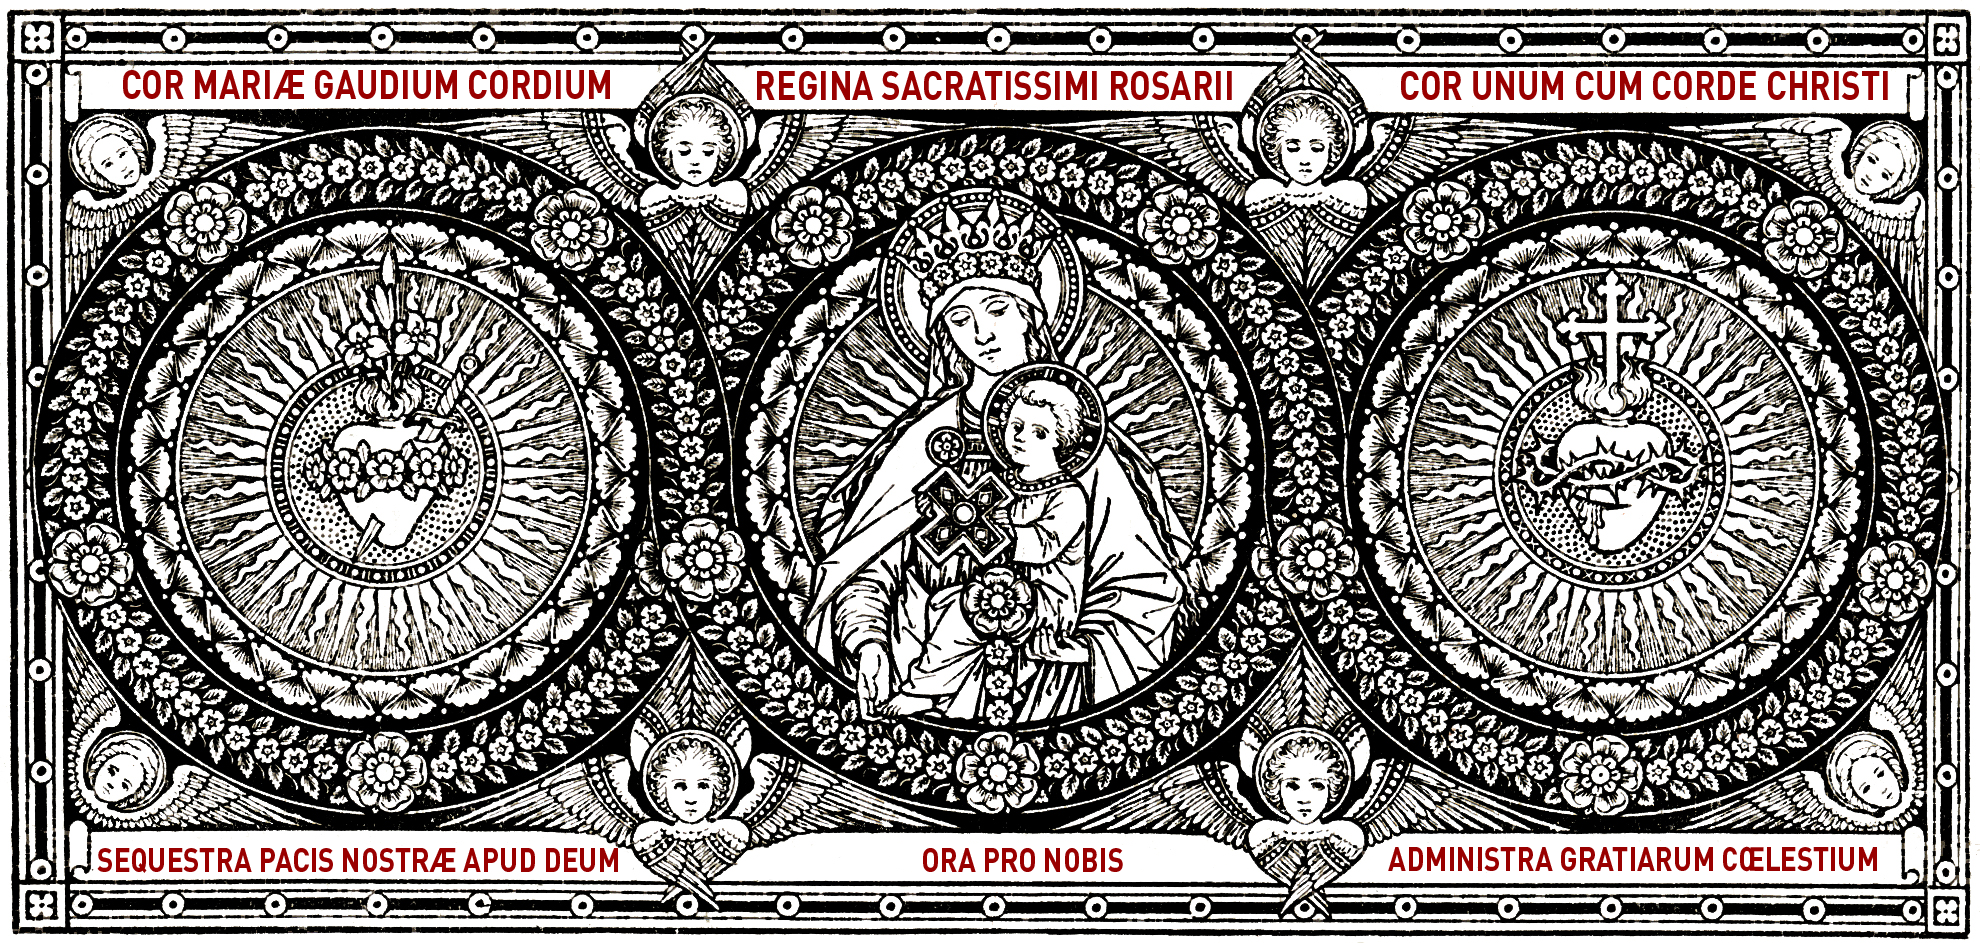
\includegraphics[width=8cm]{/img/Rosaire.png}
\end{center}
\section{Vierge de Fontpeyrine}
\lilypondfile[staffsize=15]{ly/ViergeDeFontpeyrine/ViergeDeFontpeyrine.ly}
\chanson[position=2col,numero=2,premiercouplet=2,refrain=non]{ly/ViergeDeFontpeyrine/ViergeDeFontpeyrine}
\culdelampe{3cm}{img/CulsDeLampe/cul-de-lampe.pdf}
%\lilypondfile[staffsize=15]{ly/ViergeDeFontpeyrine/ViergeDeFontpeyrine-dernier.ly}

\clearpage

\needspace{8\baselineskip}
\section{C'est le Périgord}
\lilypondfile[staffsize=15]{ly/CestLePerigord/CestLePerigord.ly}
\chanson[position=2col,numero=2,premiercouplet=2,refrain=non]{ly/CestLePerigord/CestLePerigord}

\needspace{8\baselineskip}
\section{Notre-Dame du Périgord}
\lilypondfile[staffsize=15]{ly/NotreDameDuPerigord/NotreDameDuPerigord.ly}
\chanson[numero=2,premiercouplet=2,refrain=non]{ly/NotreDameDuPerigord/NotreDameDuPerigord}

\needspace{8\baselineskip}
\section{Les saints et les anges}
\chanson[position=2col,numero=1]{ly/AveMariaDeLourdes/LesSaintsEtLesAnges}


\needspace{8\baselineskip}
\section{J'irai la voir un jour}
\chanson[position=2col,numero=1]{ly/JIraiLaVoirUnJour/JIraiLaVoirUnJour}

\needspace{8\baselineskip}
\section{Vierge sainte}
\chanson[position=2col,numero=1]{ly/ViergeSainte/ViergeSainte}

\needspace{8\baselineskip}
\section{Laudate Mariam}
\chanson[position=2col,numero=1]{ly/LaudateMariam/LaudateMariam}

\needspace{8\baselineskip}
\section{Ave Maris Stella}
\chanson[position=2col,numero=1]{ly/AveMarisStella/AveMarisStella}

\needspace{15\baselineskip}
\section{Reine de France}
\chanson[numero=1]{ly/ReineDeFrance/ReineDeFrance}

\needspace{12\baselineskip}
\section{Je mets ma confiance}
\chanson[position=2col,numero=1]{ly/JeMetsMaConfiance/JeMetsMaConfiance}

\needspace{8\baselineskip}
\section{Chez nous, soyez Reine}
\chanson[position=2col,numero=1]{ly/ChezNousSoyezReine/ChezNousSoyezReine}

\needspace{8\baselineskip}
\section{Tandis que le monde proclame}
\chanson[position=2col,numero=1]{ly/ParleCommandeRegne/ParleCommandeRegne}

\needspace{8\baselineskip}
\section{Je suis chrétien}
\chanson[position=2col,numero=1]{ly/JeSuisChretien/JeSuisChretien}

\needspace{8\baselineskip}
\section{Nous voulons Dieu}
\chanson[position=2col,numero=1]{ly/NousVoulonsDieu/NousVoulonsDieu}

\needspace{20\baselineskip}
\section{Litanies de la très sainte Vierge}
\begin{litaniae}
\invocatio{Kýrie, eléison.}{Seigneur, ayez pitié de nous.}
\invocatio{Christe, eléison.}{Jésus-Christ, ayez pitié de nous.}
\invocatio{Kýrie, eléison.}{Seigneur, ayez pitié de nous.}
\invocatio{Christe, audi nos.}{Jésus-Christ, écoutez-nous.}
\invocatio{Christe, exáudi nos.}{Jésus-Christ, exaucez-nous.}
\rinvocatio{Pater de cælis, Deus,}{Père céleste qui êtes Dieu,}{miserére nobis.}{ayez pitié de nous.}
\invocatio{Fili, Redémptor mundi, Deus,}{Fils Rédempteur du monde, qui êtes Dieu,}
\invocatio{Spíritus Sancte, Deus,}{Esprit Saint, qui êtes Dieu,}
\invocatio{Sancta Trínitas, unus Deus,}{Trinité Sainte, qui êtes un seul Dieu,}
\rinvocatio{Sancta María}{Sainte Marie}{ora pro nobis.}{priez pour nous.}
\invocatio{Sancta Dei Genitrix,}{Sainte Mère de Dieu,}
\invocatio{Sancta Virgo virginum,}{Sainte Vierge des vierges,}
\invocatio{Mater Christi,}{Mère du Christ,}
\invocatio{Mater Ecclesiae,}{Mère de la Sainte Eglise,}
\invocatio{Mater divinae gratiae,}{Mère de la divine grâce,}
\invocatio{Mater purissima,}{Mère très pure,}
\invocatio{Mater castissima,}{Mère très chaste,}
\invocatio{Mater inviolata,}{Mère toujours Vierge,}
\invocatio{Mater intemerata,}{Mère sans tache,}
\invocatio{Mater amabilis,}{Mère aimable,}
\invocatio{Mater admirabilis,}{Mère admirable,}
\invocatio{Mater boni consilii,}{Mère du bon conseil,}
\invocatio{Mater Creatoris,}{Mère du Créateur,}
\invocatio{Mater Salvatoris,}{Mère du Sauveur,}
\invocatio{Virgo prudentissima,}{Vierge très prudente,}
\invocatio{Virgo veneranda,}{Vierge vénérable,}
\invocatio{Virgo praedicanda,}{Vierge digne de louange,}
\invocatio{Virgo potens,}{Vierge puissante,}
\invocatio{Virgo clemens,}{Vierge clémente,}
\invocatio{Virgo fidelis,}{Vierge fidèle,}
\invocatio{Speculum justitiae,}{Miroir de justice,}
\invocatio{Sedes sapientiae,}{Trône de la sagesse,}
\invocatio{Causa nostrae laetiae,}{Cause de notre joie,}
\invocatio{Vas spirituale,}{Vase spirituel,}
\invocatio{Vas honorabile,}{Vase d'honneur,}
\invocatio{Vas insigne devotionis,}{Vase insigne de dévotion,}
\invocatio{Rosa mystica,}{Rose mystique,}
\invocatio{Turris Davidica,}{Tour de David,}
\invocatio{Turris ebumea,}{Tour d'ivoire,}
\invocatio{Domus aurea,}{Maison d'or,}
\invocatio{Fœderis arca,}{Arche d'alliance,}
\invocatio{Janua Caeli,}{Porte du ciel,}
\invocatio{Stella matutina,}{Étoile du matin,}
\invocatio{Salus infirmorum,}{Salut des infirmes,}
\invocatio{Refugium peccatorum,}{Refuge des pécheurs,}
\invocatio{Consolatrix afflictonim,}{Consolatrice des affligés,}
\invocatio{Auxilium Christianorum,}{Secours des chrétiens,}
\invocatio{Regina Angelorum,}{Reine des Anges,}
\invocatio{Regina Patriarcharum,}{Reine des Patriarches,}
\invocatio{Regina Prophetarum,}{Reine des Prophètes.}
\invocatio{Regina Apostolorum,}{Reine des Apôtres,}
\invocatio{Regina Martyrum,}{Reine des Martyrs,}
\invocatio{Regina Confessorum,}{Reine des Confesseurs,}
\invocatio{Regina Virginum,}{Reine des Vierges,}
\invocatio{Regina Sanctorum omnium,}{Reine de tous les Saints}
\invocatio{Regina sine labe originali concepta}{Reine conçue sans le péché originel,}
\invocatio{Regina in caelum assumpta,}{Reine élevée aux Cieux,}
\invocatio{Regina sacratissimi Rosarii,}{Reine du très saint Rosaire,}
\invocatio{Regina pacis,}{Reine de la paix,}
\rinvocatio{Agnus Dei, qui tollis peccáta mundi,}{Agneau de Dieu, qui effacez les péchés du monde,}%
{parce nobis, Dómine.}{pardonnez-nous, Seigneur.}
\rinvocatio{Agnus Dei, qui tollis peccáta mundi,}{Agneau de Dieu, qui effacez les péchés du monde,}%
{exáudi nos, Dómine.}{exaucez-nous, Seigneur.}
\rinvocatio{Agnus Dei, qui tollis peccáta mundi,}{Agneau de Dieu, qui effacez les péchés du monde,}%
{miserére nobis.}{ayez pitié de nous.}
\end{litaniae}
\versio{\vb. Ora pro nobis, sancta Dei Génetrix,}{Priez pour nous sainte Mère de Dieu}
\versio{\rb. Ut digni efficiámur promissiónibus Christi.}{Afin que nous soyons dignes des promesses du Christ}
\versio{\centering{Orémus}

Concéde nos fámulos tuos, quǽsumus, Dómine Deus, perpétua mentis et córporis sanitáte gaudére : et, gloriósa beátæ Maríæ semper Vírginis intercessióne, a præsénti liberári tristítia et ætérna pérfrui lætítia. Per Dóminum.}
{\centering{Prions.}

Seigneur, daignez nous accorder, à nous vos serviteurs, de jouir toujours de la santé de l'âme et du corps; et par la glorieuse intercession de la bienheureuse Marie toujours Vierge, délivrez-nous des tristesses de la vie présente, et donnez-nous d'avoir part aux joies éternelles. Par Jésus-Christ Notre Seigneur.}
\culdelampe{5cm}{img/CulsDeLampe/rosace-4.pdf}


%%%%%%%%%%%%%%%%%%%%%%%%%%%%%%%%%%%%%%%%%%%%%%%%%%%%%%%%%%%%%%%%%%%%%%%%%%%%%%%%
\addchap{Ordinaire de la Messe}
\label{Ordo}
\culdelampe{\textwidth}{img/Missa.jpg}
\vspace{-.7\baselineskip}
\subsection*{Prières au bas de l'autel}\blindsection{Messe des catéchumènes}
\vspace{-.3\baselineskip}

\rubrica{Le prêtre et les ministres qui l'assistent se préparent à la célébration de la Liturgie par les prières dites au bas de l'autel. À la messe chantée elles sont dites à voix basse ; on se reporte directement à l'Introït.}

\versio{%
In nómine Patris, et Fílii, et Spíritus Sancti. Amen.}{%
Au nom du Père, et du Fils, et du Saint-Esprit. Ainsi soit-il.}

\versio{%
℣. Introíbo ad altáre Dei.}{%
℣. Je monterai à l'autel de Dieu.}

\versio{%
℟. Ad Deum, qui lætíficat iuventútem meam.}{%
℟. Jusqu'au Dieu qui réjouit ma jeunesse.}

\versio{%
℣. Iúdica me, Deus, et discérne causam meam de gente non sancta : ab hómine iníquo et dolóso érue me.}{%
℣. Jugez-moi, ô Dieu, et distinguez ma cause de celles de la nation impie : arrachez-moi de l'homme inique et trompeur.}

\versio{%
℟. Quia tu es, Deus, fortitúdo mea : quare me repulísti, et quare tristis incédo, dum afflígit me inimícus ?}{%
℟. Car, ô Dieu, vous êtes ma force : pourquoi m'avez-vous repoussé, et m'en vais-je triste, tandis que l'ennemi m'af\-flige ?\looseness=-1}

\versio{%
℣. Emítte lucem tuam et veritátem tuam : ipsa me deduxérunt et adduxérunt in montem sanctum tuum, et in tabernácula tua.\looseness=-1}{%
℣. Envoyez votre lumière et votre vérité : elles m'ont conduit et m'ont amené à votre montagne sainte et dans vos palais.}

\versio{%
℟. Et introíbo ad altáre Dei : ad Deum qui lætíficat iuventútem meam.}{%
℟. Et je monterai à l'autel de Dieu, jusqu'au Dieu qui réjouit ma jeunesse.}

\versio{%
℣. Confitébor tibi in cíthara, Deus, Deus meus : quare tristis es anima mea, et quare contúrbas me ?}{%
℣. Je vous louerai sur la harpe, ô Dieu, mon Dieu : pourquoi es-tu triste, ô mon âme, et pourquoi me troubles-tu ?\looseness=-1}

\versio{%
℟. Spera in Deo, quóniam adhuc confitébor illi : salutáre vultus mei, et Deus meus.}{%
℟. Espère en Dieu, parce que je le louerai encore : il est le salut de mon visage et il est mon Dieu.}

\versio{%
℣. Glória Patri, et Fílio, et Spirítui Sancto.}{%
℣. Gloire au Père, et au Fils, et au Saint-Esprit.}%

\versio
{
℟. Comme il était au commencement, maintenant, et toujours, et dans les siècles des siècles. Ainsi \mbox{soit-il.}}

\versio{%
℣. Introíbo ad altáre Dei.}{%
℣. Je monterai à l'autel de Dieu.}

\versio{%
℟. Ad Deum qui lætíficat iuventútem meam.}{%
℟. Jusqu'au Dieu qui réjouit ma jeunesse.}

\versio{%
℣. Adiutórium nostrum in nómine Dómini.}{%
℣. Notre secours est dans le nom du Seigneur.}

\versio{%
℟. Qui fecit cælum et terram.}{%
℟. Qui a fait le ciel et la terre.}

\rubrica{%
Le célébrant récite le \emph{Confiteor}, puis les ministres (et les fidèles à la messe lue) répondent :%
}

\versio{%
℟. Misereátur tui omnípotens Deus, et dimissis peccátis tuis, perdúcat te ad vitam ætérnam.}{%
℟. Que le Dieu tout-puissant vous fasse miséricorde, vous pardonne vos péchés, et vous con\-duise à la vie \mbox{éternelle.}}

\versio{%
℣. Amen.}{%
℣. Ainsi soit-il.}

\rubrica{%
Les ministres récitent alors le \emph{Confiteor} :%
}

\versio{%
Confíteor Deo omnipoténti, beá\-tæ Maríæ semper Vírgini, beáto Michaéli Archángelo, beáto Ioánni Baptístæ, sanctis Apóstolis Petro et Páulo, ómnibus Sanctis, et tibi pater : quia peccávi nimis cogitatióne, verbo, et ópere : mea culpa, mea culpa, mea máxima culpa. Ideo precor beátam Maríam semper Vírginem, beátum Michaélem Archángelum, beátum Ioánnem Baptístam, sanctos Apóstolos Petrum et Páulum, omnes Sanctos, et te, pater, oráre pro me ad Dóminum Deum nostrum.}{%
Je confesse à Dieu tout-puissant, à la bienheureuse Marie toujours vierge, à saint Michel Archange, à saint Jean-Baptiste, aux saints Apôtres Pierre et Paul, à tous les saints et à vous mon père, que j'ai beaucoup péché, par pensées, par paroles et par actions. C'est ma faute, c'est ma faute, c'est ma très grande faute. C'est pourquoi je supplie la bienheureuse Marie toujours vierge, saint Michel Archange, saint Jean-Baptiste, les saints Apôtres Pierre et Paul, tous les saints et vous mon père, de prier pour moi le Seigneur notre Dieu.}


\versio{%
℣. Misereátur vestri omnípotens Deus, et dimíssis peccátis vestris, perdúcat vos ad vitam ætérnam.}{%
℣. Que le Dieu tout-puissant vous fasse miséricorde, qu'il vous pardonne vos péchés et vous con\-duise à la vie éternelle.}

\versio{%
℟. Amen.}{%
℟. Ainsi soit-il.}

\versio{%
℣. Indulgéntiam, absolutiónem, et remissiónem peccatórum nostrórum, tríbuat nobis omnípotens et miséricors Dóminus.}{%
℣. Que le Dieu tout-puissant et miséricordieux nous accorde le pardon, l'absolution et la rémission de nos péchés.}

\versio{%
℟. Amen.}{%
℟. Ainsi soit-il.}

\versio{%
℣. Deus, tu convérsus vivificábis nos.}{%
℣. Dieu, tournez-vous vers nous et donnez-nous la vie.}

\versio{%
℟. Et plebs tua lætábitur in te.}{%
℟. Votre peuple se réjouira en vous.\looseness=-1}

\versio{%
℣. Osténde nobis Dómine, misericórdiam tuam.}{%
℣. Montrez-nous, Seigneur, votre miséricorde.}

\versio{%
℟. Et salutáre tuum da nobis.}{%
℟. Accordez-nous votre salut.}

\versio{%
℣. Dómine, exáudi oratiónem meam.\looseness=-1}{%
℣. Seigneur, exaucez ma prière.}

\versio{%
℟. Et clamor meus ad te véniat.}{%
℟. Que mon appel vous parvienne.\looseness=-1}

\versio{%
℣. Dóminus vobíscum.}{%
℣. Le Seigneur soit avec vous.}

\versio{%
℟. Et cum spíritu tuo.}{%
℟. Et avec votre esprit.}

\medskip

\versio{%
Orémus.}{%
Prions.}

\needspace{5\baselineskip}
\subsection*{Montée à l'autel}

\rubrica{En montant à l'autel le prêtre dit la prière suivante :}

\versio{%
Aufer a nobis, quǽsumus, Dómine, iniquitátes nostras : ut ad Sancta sanctórum puris mereámur méntibus introíre. Per Christum Dóminum no\-strum. Amen.}{%
Enlevez nos fautes, Seigneur, pour que nous puissions pénétrer dans le Saint des Saints avec une âme pure. Par le Christ notre Seigneur. Ainsi soit-il.}

%\smallskip\needspace{\baselineskip}
\rubrica{L'autel, en pierre, représente le Christ : \emph{il est la pierre vivante choisie par Dieu} (I~Pierre, 2,4). Cette pierre contient les reliques des martyrs qui ont versé leur sang pour le Christ. En la baisant le prêtre adore le Christ et vénère les saints martyrs.}

\versio{%
Orámus te, Dómine, per mérita Sanctórum tuórum, quorum relíquiæ hic sunt, et ómnium Sanctórum : ut indúlgere dignéris ómnia peccáta mea. Amen.}{%
Nous vous en prions, Seigneur, par les mérites de vos saints (il baise l'autel au milieu) dont nous avons ici les reliques et de tous les saints, daignez pardonner tous mes péchés. Ainsi soit-il.}

\needspace{3\baselineskip}
\rubrica{Le Prêtre bénit l'encens, en disant :}

\versio{%
Ab illo bene~✠ dicáris, in cuius honóre cremáberis. Amen.}{%
Sois bé~✠ ni par celui en l'honneur de qui tu vas brûler. Ainsi soit-il.}

\rubrica{Et ayant reçu l'encensoir du diacre, il encense l'autel, sans rien dire. Puis le diacre, ayant reçu l'encensoir du Prêtre, encense ce dernier.}


\subsection*{Avant-messe}

\rubrica{La première partie de la Liturgie est appelée "Avant-messe" ou "messe des catéchumènes". Elle est une préparation au saint Sacrifice et consiste dans un ensemble de prières, de chants et de lectures de la Sainte Écriture. Chaque jour liturgique a un thème ou une orientation spirituelle particulière qui y est exprimée. \emph{Les chants sacrés qui résument les plus saintes vérités préparent harmonieusement nos âmes aux mystères que nous devons célébrer. Ils nous mettent à l'unisson des chants divins et nous accordent aux réalités divines, avec nous-mêmes et les uns aux autres : nous ne formons plus qu'un chœur unique et homogène d'hommes saints}. (Denys l'Aréopagite)}


\subsection*{%
Introït%
}

\rubrica{Voir au propre du jour.}


\subsection*{%
Kyrie%
}
\rubrica{Le chant du Kyrie et du Gloria se trouvent à partir de la page \pageref{Kyriale}}

\rubrica{Le Kyrie est le reste d'une litanie plus longue, qui était toujours chantée en grec. Le diacre formulait des intentions et on répondait : Seigneur, ayez pitié. De cette litanie il ne reste aujourd'hui que neuf invocations, trois pour chaque personne de la Sainte Trinité. Nous recommandons à Dieu les besoins de l'Église et nos intentions personnelles.}

\versio{%
Kýrie, eléison. \emph{ter}

Christe, eléison. \emph{ter}

Kýrie, eléison. \emph{ter}%
}{%
Seigneur, ayez pitié. \emph{ter}

Christ, ayez pitié. \emph{ter}

Seigneur, ayez pitié. \emph{ter}%
}%


\needspace{5\baselineskip}
\subsection*{%
Gloria%
}%

\rubrica{Le Gloria faisait partie de l'office de nuit et fut progressivement introduit dans la messe à partir du V\ieme\ siècle. C'est un développement du chant des anges dans la nuit de Noël. C'est la grande glorification du Dieu trinitaire : Gloire au Père, au Fils et au Saint-Esprit.}

\versio{%
Glória in excélsis Deo. Et in terra pax homínibus bonæ voluntátis. Laudámus te. Benedícimus te. Adorámus te. Glorificámus te. Grátias ágimus tibi propter magnam glóriam tuam. Dómine Deus, Rex cæléstis, Deus Pater omnípotens. Dómine Fili unigénite, Iesu Christe. Dómine Deus, Agnus Dei, Fílius Patris. Qui tollis peccáta mundi, miserére nobis. Qui tollis peccáta mundi, súscipe deprecatiónem nostram. Qui sedes ad déxteram Patris, miserére nobis. Quóniam tu solus Sanctus. Tu solus Dóminus. Tu solus Altíssimus, Iesu Christe. Cum Sancto Spíritu in glória Dei Patris. Amen.%
}{%
Gloire à Dieu au plus haut des cieux, et paix sur la terre aux hommes de bonne volonté. Nous vous louons, nous vous bénissons, nous vous adorons, nous vous glorifions. Nous vous rendons grâces pour votre gloire immense, Seigneur Dieu, Roi du ciel, Dieu Père tout-puissant. Seigneur Fils unique, Jésus-Christ, Seigneur Dieu, Agneau de Dieu, Fils du Père, vous qui enlevez les péchés du monde, ayez pitié de nous ; vous qui enlevez les péchés du monde, accueillez notre prière ; vous qui siégez à la droite du Père, ayez pitié de nous. Car vous êtes le seul Saint, le seul Seigneur, le seul Très-Haut, Jésus-Christ, avec le Saint-Esprit, dans la gloire de Dieu le Père. Ainsi soit-il.\looseness=-1%
}%


\subsection*{Collecte}

\rubrica{Le prêtre se tourne vers les fidèles pour les saluer et les inviter à s'unir à la prière qu'il va prononcer en leur nom.}

\versio{%
℣. Dóminus vobíscum.}{%
℣. Le Seigneur soit avec vous.}

\versio{%
℟. Et cum spíritu tuo.}{%
℟. Et avec votre esprit.}

\rubrica{La Collecte chantée par le prêtre exprime l'intention de la prière de l'Église en ce jour et la grâce spéciale qu'elle demande. Cette oraison est répétée plusieurs fois au cours de l'office. Le prêtre la prononce les mains élevées comme pour diriger la prière vers le ciel ; dans la Sainte Écriture élever les mains est synonyme de prier. On se tient debout, sauf les jours de pénitence et aux messes des défunts, où l'on est à genoux.}

%\medskip\pagebreak[1]

\versio{%
Orémus.}{%
Prions.}

\rubrica{Voir au propre du jour. À la fin de la collecte, on répond :}

\versio{%
℟. Amen.}{%
℟. Ainsi soit-il.}


\needspace{5\baselineskip}
\subsection*{Épître}

\rubrica{Les lectures ne suivent pas l'ordre des livres de la Bible, mais l'Église a choisi les textes les plus importants en rapport avec le temps liturgique ou le mystère célébré en ce jour.}

\rubrica{Voir à la Messe du jour.}

\rubrica{À la messe lue on répond :}

\versio{%
℟. Deo grátias.}{%
℟. Rendons grâces à Dieu.}%


\subsection*{Graduel, Alléluia et Séquence}

\rubrica{Graduel, Alléluia sont des chants de méditation sur les lectures ou le mystère liturgique de ce jour. \emph{Alleluia} signifie "louez Dieu". L'Alléluia se prolonge dans une mélodie ornée qui exprime la joie spirituelle au-delà des paroles.}

\rubrica{Voir au propre du jour.}

\needspace{5\baselineskip}
\subsection*{%
Évangile%
}

\rubrica{On chante le saint Évangile tourné vers le Nord (le chœur étant normalement orienté vers l'Est) parce que le Nord symbolise les âmes qui se trouvent dans la froideur de l'infidélité et de l'ignorance du Christ, et qui sont éveillées par le souffle du Saint-Esprit.}

\versio{%
℣. Dóminus vobíscum.}{%
℣. Le Seigneur soit avec vous.}

\versio{%
℟. Et cum spíritu tuo.}{%
℟. Et avec votre esprit.}

\needspace{3\baselineskip}
\rubrica{Voir au propre du jour. À la messe lue on répond :}

\versio{%
℟. Laus tibi, Christe.}{%
℟. Louange à vous, ô Christ.}


\subsection*{%
Credo%
}

\versio{%
Credo in Deum, Patrem omnipoténtem, factórem cæli et terræ, visibilium omnium et invisibilium.

Et in unum Dóminum Iesum Christum, Fílium Dei unigenitum. Et ex Patre natum ante ómnia sǽcula. Deum de Deo, lumen de lúmine, Deum verum de Deo vero. Génitum, non factum, consubstantiálem Patri : per quem ómnia facta sunt. Qui propter nos hómines et propter nostram salútem descéndit de cælis. Et incarnátus est de Spíritu Sancto ex María Vírgine : et homo factus est. Crucifíxus étiam pro nobis : sub Póntio Piláto passus, et sepúltus est. Et resurréxit tértia die, secúndum Scriptúras. Et ascéndit in cælum : sedet ad déxteram Patris. Et iterum ventúrus est cum glória iudicáre vivos et mórtuos : cuius regni non erit finis.\looseness=-1

Et in Spíritum Sanctum, Dóminum, et vivificántem : qui ex Patre Filióque procédit. Qui cum Patre et Fílio simul adorátur et conglorificátur : qui locútus est per Prophétas.

Et unam, sanctam, cathólicam et apostólicam Ecclésiam. Confíteor unum baptísma in remissiónem peccatórum. Et exspécto resurrectiónem mortuórum. Et vitam ventúri sǽculi. Amen.%
}{%
  Je crois en un seul Dieu, le Père tout-puissant, créateur du ciel et de la terre, de toutes choses, visibles et invisibles.

  Je crois en un seul Seigneur Jésus-Christ, le Fils unique de Dieu, né du Père avant tous les siècles ; Dieu né de Dieu, lumière née de la lumière, vrai Dieu né du vrai Dieu. Engendré, non pas créé, consubstantiel au Père, et par qui tout a été créé. C'est lui qui, pour nous les hommes, et pour notre salut, est descendu des cieux. Il a pris chair de la Vierge Marie par l'action du Saint-Esprit, et il s'est fait homme. Puis il fut crucifié pour nous sous Ponce-Pilate : il souffrit et fut mis au tombeau. Il ressuscita le troisième jour, suivant les Ecritures. Il monta aux cieux, où il siège à la droite du Père. De nouveau il viendra dans la gloire pour juger les vivants et les morts, et son règne n'aura pas de fin.

  Je crois en l'Esprit-Saint, qui est Seigneur et qui donne la vie, qui procède du Père et du Fils. Avec le Père et le Fils, il reçoit même adoration et même gloire. Il a parlé par les prophètes.

  Je crois à l'Église une, sainte, catholique et apostolique. Je reconnais un seul Baptême pour la rémission des péchés, et j'attends la résurrection des morts et la vie du monde à venir. Ainsi soit-il.
}

\culdelampe{5cm}{img/CulsDeLampe/separateur-texte.pdf}
\needspace{10\baselineskip}
\subsection*{%
Offertoire%
}\blindsection{Offertoire}

\rubrica{À l'Offertoire l'Église offre le Corps et le Sang du Christ, représentés par le pain et le vin. Notre Seigneur a communiqué à son Église le pouvoir d'offrir le même sacrifice qu'il offrit sur la Croix. L'Église s'y unit comme victime. \emph{Le Christ lui-même est à la fois le prêtre qui offre et la victime qui est offerte. Le sacrifice de l'Église est le sacrement quotidien du sacrifice du Christ. L'Église, qui est le corps dont il est la tête, s'y offre elle-même par lui. C'est pourquoi dans ce sacrement l'Église elle-même est offerte dans ce qu'elle offre.} (S.~Augustin). Nous sommes donc une seule victime avec le Christ, unissant nos propres offrandes et nos sacrifices à celui du Christ et de l'Église. Notre participation à cette offrande est exprimée par le chant de l'offertoire.}

\versio{%
℣. Dóminus vobíscum.}{%
℣. Le Seigneur soit avec vous.}

\versio{%
℟. Et cum spíritu tuo.}{%
℟. Et avec votre esprit.}

\medskip

\versio{%
Orémus.}{%
Prions.}


\vspace{-.6\baselineskip}
\subsection*{Antienne d'offertoire}


\rubrica{Voir au propre du jour.}


\vspace{-.6\baselineskip}
\subsection*{Offrande du pain}

\versio{%
Súscipe, sancte Pater, omnípotens ætérne Deus, hanc immaculátam hóstiam, quam ego indígnus fámulus tuus óffero tibi Deo meo, vivo et vero, pro innumerabílibus peccátis, et offensiónibus, et negligéntiis meis, et pro ómnibus circumstántibus, sed et pro ómnibus fidélibus christiánis vivis atque defúnctis : ut mihi et illis profíciat ad salútem in vitam ætérnam. Amen.}{%
Recevez, Père saint, Dieu éternel et tout-puissant, cette offrande sans tache, que moi, votre indigne serviteur, je vous présente, à vous, mon Dieu vivant et vrai, pour mes péchés, offenses et négligences sans nombre, pour tous ceux qui m'entourent, ainsi que pour tous les fidèles vivants et morts : qu'elle serve à mon salut et au leur pour la vie éternelle. Ainsi soit-il.}

\vspace{-.8\baselineskip}
\subsection*{Préparation et offrande du vin}

\rubrica{Le diacre prépare le calice en y versant le vin ; le sous-diacre y ajoute quelques gouttes d'eau que le prêtre bénit (s'il est seul le prêtre accomplit lui-même ces cérémonies). L'eau mêlée au vin figure l'union en Jésus-Christ de la nature humaine à la personne divine, et symbolise aussi le chrétien intimement uni au Christ. Le vin et l'eau rappellent le Sang et l'eau qui coulèrent du côté du Christ percé par la lance. \emph{Quand le vin et l'eau sont mêlés dans le calice, le peuple est uni au Christ et la foule des croyants est associée et réunie à celui en qui elle croit.} (S.~Cyprien)}

\versio{%\widowpenalty=10000%
Deus,~✠ qui humánæ substántiæ dignitátem mirabíliter condidísti, et mirabílius reformásti : da nobis, per huius aquæ et vini mystérium, eius divinitátis esse consórtes, qui humanitátis nostræ fíeri dignátus est párticeps, Iesus Christus, Fílius tuus, Dóminus noster : Qui tecum vivit et regnat in unitáte Spíritus Sancti Deus : per ómnia sǽcula sæculórum. Amen.\looseness=1%
}{%\widowpenalty=10000%
Dieu,~✠ qui, d'une manière admirable, avez créé la nature humaine dans sa noblesse, et l'avez restaurée d'une manière plus admirable encore, accordez-nous, selon le mystère de cette eau et de ce vin, de prendre part à la divinité de celui qui a daigné partager notre humanité, Jésus-Christ votre Fils, Notre Seigneur, qui, étant Dieu, vit et règne avec vous en l'unité du Saint-Esprit, dans tous les siècles des siècles. \mbox{Ainsi soit-il}.\looseness=1}

\versio{%
Offérimus tibi, Dómine, cálicem salutáris, tuam deprecántes cleméntiam : ut in conspéctu divínæ maiestátis tuæ, pro nostra et totíus mundi salúte, cum odóre suavitátis ascéndat. Amen.}{%
Nous vous offrons, Seigneur, le calice du salut, et nous demandons à votre clémence qu'il s'élève en parfum agréable devant votre divine Majesté, pour notre salut et celui du monde entier. Ainsi soit-il.}

\versio{%
In spíritu humilitátis, et in ánimo contríto suscipiámur a te, Dómine : et sic fiat sacrifícium nostrum in conspéctu tuo hódie, ut pláceat tibi, \mbox{Dómine Deus.}}{%
Voyez l'humilité de nos âmes et la contrition de nos cœurs : accueillez-nous, Seigneur, et que notre sacrifice s'accomplisse aujourd'hui devant vous de telle manière qu'il vous soit agréable, Seigneur Dieu.}

\versio{%
Veni, sanctificátor, omnípotens ætérne Deus : et béne~✠ dic hoc sacrifícium, tuo sancto nómini præparátum.}{%
Venez, Sanctificateur, Dieu éternel et tout-puissant, et~✠ bénissez ce sacrifice préparé pour votre saint Nom.}

\needspace{10\baselineskip}
\subsection*{Encensement}

\rubrica{Comme l'encens, consumé par le feu, s'élève en vapeur odorante, ainsi l'Église avec le Christ, consumée par le feu du Saint-Esprit, s'élève en sacrifice envers Dieu. On encense les oblats (le pain et le vin), puis l'autel, le prêtre, et enfin le clergé et les fidèles.}

\versio{%
Per intercessiónem beáti Michaélis archángeli, stantis a dextris altáris incénsi, et ómnium electórum suórum, incénsum istud dignétur Dóminus bene~✠ dícere, et in odórem suavitátis accípere. Per Christum Dóminum nostrum. Amen.}{%
Par l'intercession de l'archange saint Michel, qui se tient à droite de l'autel de l'encens, et par l'intercession de tous ses élus, que le Seigneur daigne bénir~✠ cet encens, et le recevoir comme un parfum agréable. Par le Christ notre Seigneur. Ainsi soit-il.}

\versio{%
Incénsum istud, a te benedíctum, ascéndat ad te, Dómine : et descéndat super nos misericórdia tua. }{%
Que cet encens béni par vous, Seigneur, monte vers vous, et que descende sur nous votre miséricorde.}

\versio{%
Dirigátur, Dómine, orátio mea, sicut incénsum, in conspéctu tuo : elevátio mánuum meárum sacrifícium vespertínum. Pone, Dómine, custódiam ori meo, et óstium circumstántiæ lábiis meis : ut non declínet cor meum in verba malítiæ, ad excusándas excusatiónes in peccátis.}{%
Seigneur, que ma prière s'élève comme l'encens devant votre face ; que mes mains levées soient comme l'offrande du soir. Placez, Seigneur, une garde à ma bouche et une barrière tout autour de mes lèvres. Que mon cœur ne se porte pas à des paroles mauvaises qui servent de \mbox{prétexte au péché. (Ps. 140)}}

\versio{%
Accéndat in nobis Dóminus ignem sui amóris, et flammam ætérnæ caritátis. Amen.}{%
Que le Seigneur allume en nous le feu de son amour et la flamme de l'éternelle charité. Ainsi soit-il.}


\subsection*{Lavabo}

\rubrica{\emph{Les mains sont le symbole de l'action. En les lavant nous signifions la pureté et l'innocence des actions.} (S.~Cyprien)}

\versio{%
Lavábo inter innocéntes manus meas : et circúmdabo altáre tuum, Dómine : Ut áudiam vocem laudis, et enárrem univérsa mirabília tua. Dómine, diléxi decórem domus tuæ, et locum habitatiónis glóriæ tuæ. Ne perdas cum ímpiis, Deus, ánimam meam, et cum viris sánguinum vitam meam : In quorum mánibus iniquitátes sunt : déxtera eórum repléta est munéribus. Ego autem in innocéntia mea ingréssus sum : rédime me, et miserére mei. Pes meus stetit in dirécto : in ecclésiis benedícam te, Dómine. Glória Patri, et Fílio, et Spirítui Sancto, Sicut erat in princípio, et nunc, et semper, et in sǽcula sæculórum. Amen.}{%
Je laverai mes mains parmi les innocents, et je me tiendrai devant votre autel, Seigneur. Pour entendre la voix de la louange et raconter toutes vos merveilles. Seigneur, j'aime la beauté de votre maison et le lieu où réside votre gloire. Ô Dieu, ne condamnez pas mon âme avec celle des impies ; ne m'enlevez pas la vie comme aux hommes de sang. Leurs mains commettent l'iniquité, et leur droite est comblée de présents.
Pour moi je marche dans l'innocence ; rachetez-moi et ayez pitié de moi. Mon pied se tient dans la voie droite ; je vous bénirai, Seigneur, dans l'assemblée. Gloire au Père, au Fils, et au Saint-Esprit. Comme il était au commencement, maintenant et toujours, et dans tous les siècles des siècles. Ainsi soit-il.}


%\vfill\pagebreak[0]

\subsection*{Prière à la Sainte Trinité}

\versio{%
Súscipe, sancta Trínitas, hanc oblatiónem, quam tibi offérimus ob memóriam passiónis, resurrectiónis, et ascensiónis Iesu Christi Dómini nostri : et in honórem beátæ Maríæ semper Vírginis, et beáti Ioánnis Baptístæ, et sanctórum Apostolórum Petri et Pauli, et istórum, et ómnium sanctórum : ut illis profíciat ad honórem, nobis autem ad salútem : et illi pro nobis intercédere dignéntur in cælis, quorum memóriam ágimus in terris. Per eúndem Christum Dóminum nostrum. Amen.}{%
Recevez, Trinité Sainte, cette of\-frande que nous vous présentons en mémoire de la Passion, de la Résurrection et de l'Ascension de Jésus-Christ notre Seigneur, en l'honneur aussi de la bienheureuse Marie toujours vierge, de saint Jean-Baptiste, des saints Apôtres Pierre et Paul, des saints dont les reliques sont ici, et de tous les saints. Qu'elle soit pour eux une source d'honneur, et pour nous une cause de salut, et qu'ils daignent intercéder pour nous au ciel, eux dont nous célébrons la mémoire sur terre. Par le Christ notre Seigneur. Ainsi soit-il.\looseness=-1}

\needspace{3\baselineskip}
\rubrica{Le prêtre dit, tourné vers les fidèles :}

\versio{%
Oráte, fratres : ut meum ac vestrum sacrifícium acceptábile fiat apud Deum Patrem omnipoténtem.}{%
Priez, mes frères, pour que mon sacrifice, qui est aussi le vôtre, puisse être agréé par Dieu le Père tout-puissant.}

\rubrica{À la messe lue on répond :}

\versio{%
℟. Suscípiat Dóminus sacrifícium de mánibus tuis, ad laudem et glóriam nóminis sui, ad utilitátem quoque nostram, totiúsque Ecclésiæ suæ sanctæ.}{%
℟. Que le Seigneur reçoive de vos mains le sacrifice, à la louange et à la gloire de son Nom, ainsi que pour notre bien et celui de toute sa sainte Église.}


\subsection*{%
Secrète%
}

\rubrica{Voir au propre du jour.}

\needspace{5\baselineskip}
\subsection*{Oblation du Sacrifice}

\rubrica{Commence ici la partie la plus sacrée de la Liturgie : le sacrifice réel et sacramentel où le prêtre immole le Christ. \emph{Vraiment à cette heure très redoutable il faut tenir haut son cœur vers Dieu, et non en bas vers la terre et les affaires terrestres. D'autorité donc le pontife  enjoint à cette heure à tous de laisser de côté les soucis, les sollicitudes domestiques, et de tenir leur cœur au ciel vers Dieu ami des hommes.} \mbox{(S. Cyrille de Jérusalem)}}


\subsection*{%
Préface%
}


\rubrica{Par le chant de la Préface le prêtre rend grâces à Dieu au nom de l'Église pour l'œuvre du salut réalisée par Jésus-Christ.}

\versio{%
℣. Per ómnia sǽcula sæculórum. ℟. Amen.}{%
℣. Dans tous les siècles des siècles. ℟. Ainsi soit-il.}

\versio{%
℣. Dóminus vobíscum.}{%
℣. Le Seigneur soit avec vous.}

\versio{%
℟. Et cum spíritu tuo.}{%
℟. Et avec votre esprit.}

\versio{%
℣. Sursum corda.}{%
℣. Élevons nos cœurs.}

\versio{%
℟. Habémus ad Dóminum.}{%
℟. Ils sont tournés vers le Seigneur.\looseness=-1}

\versio{%
℣. Grátias agámus Dómino Deo nostro.}{%
℣. Rendons grâces au Seigneur notre Dieu.}

\versio{%
℟. Dignum et iustum est.}{%
℟. C'est juste et nécessaire.}

\versio{%
Vere dignum et iustum est,
æquum et salutáre,
nos tibi semper et ubíque grátias ágere :
Dómine, sancte Pater, omnípotens ætérne Deus :
}{%
Il est vraiment juste et nécessaire,
c'est notre devoir et c'est notre salut,
de vous rendre grâces toujours et partout,
Seigneur, Père saint, Dieu éternel et tout-puissant :%
}
\versio{%
Et te in Visitatióne \emph{\rubrum{vel}} Assumptióne \emph{\rubrum{vel}} Nativitáte beátæ Maríæ semper Vírginis
collaudáre, benedícere et prædicáre.
Quæ et Unigénitum tuum Sancti Spíritus obumbratióne concépit :
et, virginitátis glória permanénte,
lumen ætérnum mundo effúdit,
Iesum Christum, Dóminum nostrum.

Per quem maiestátem tuam laudant Angeli,
adórant Dominatiónes,
tremunt Potestátes.
Cæli cælorúmque Virtútes ac beáta Séraphim
sócia exsultatióne concélebrant.
Cum quibus et nostras voces ut admítti iúbeas, deprecámur,
súpplici confessióne dicentes.%
}{%
Et, en la Visitation \emph{\rubrum{ou}} l'Assomption \emph{\rubrum{ou}} la Nativité de la bienheureuse Marie toujours Vierge
de vous louer, de vous bénir et de vous proclamer.
C'est elle qui a conçu votre Fils unique par l'opération du Saint-Esprit :
et qui, sans rien perdre de la gloire de sa virginité,
a mis au monde la lumière éternelle,
Jésus-Christ, Notre-Seigneur.

Par Lui les Anges louent votre majesté,
les Dominations vous adorent,
les Puissances se prosternent en tremblant.
Les Cieux, les Vertus des cieux et les bienheureux Séraphins
la célèbrent, unis dans une même allégresse.
À leurs chants, nous vous prions, laissez se joindre aussi nos voix
pour proclamer dans une humble louange.%
}

\needspace{9\baselineskip}
\subsection*{%
Sanctus%
}

\rubrica{L'hymne au Dieu trois fois saint se compose d'une vision du prophète Isaïe (Is. 6,3) et des acclamations chantées lors de l'entrée triomphale du Christ à Jérusalem. Le sacrifice du Christ s'achève par sa résurrection et son ascension : Notre-Seigneur entre triomphalement dans la Jérusalem céleste. \emph{Le Christ est entré une fois pour toutes dans le sanctuaire du ciel avec son propre Sang, nous ayant acquis une rédemption éternelle.} (Hébreux 9,12). \emph{Nous chantons cette glorification qui nous a été transmise des Séraphins, pour que, en communiant  à cette hymne, nous soyons unis aux armées angéliques.} (S.~Cyrille de Jérusalem)}

\rubrica{Le chant du Sanctus se trouve à partir de la page \pageref{Kyriale}}

\versio{%
Sanctus, sanctus, sanctus Dóminus, Deus Sábaoth. Pleni sunt cæli et terra glória tua. Hosánna in excélsis ! Benedíctus qui venit in nómine Dómini. Hosánna in excélsis~!%
}{%
Saint, saint, saint le Seigneur, Dieu des armées. Les cieux et la terre sont remplis de votre gloire ; hosanna au plus haut des cieux ! Béni soit celui qui vient au nom du Seigneur ; hosanna au plus haut des cieux !%
}%

\clearpage
\needspace{4\baselineskip}
\subsection*{Canon}\blindsection{Canon}
\culdelampe{\textwidth}{img/Canon.jpg}
\rubrica{Canon signifie règle. Cette partie de la messe est une règle intangible. Les prières du Canon remontent au-delà du VI\ieme{} siècle, voire pour certaines à l'Apôtre Pierre lui-même.}

\rubrica{Jusqu'à la fin du Canon le silence le plus complet règne dans l'église. Le prêtre "entre" dans le saint des saints de la Liturgie. Dans les premiers siècles un rideau dérobait le prêtre à la vue de l'assemblée. Depuis le XI\ieme{} siècle le Canon est dit à voix basse par respect et vénération et aussi parce que le prêtre seul, de par son caractère sacerdotal, a le pouvoir de le prononcer et d'accomplir le sacrifice par la consécration du pain et du vin au Corps et au Sang du Christ.}

\versio{%
Te ígitur, clementíssime Pater, per Iesum Christum Fílium tuum Dóminum nostrum, súpplices rogámus, ac pétimus, uti accépta hábeas, et bene\-dícas hæc~✠ dona, hæc~✠ mún\-era, hæc sancta~✠ sacrifícia illibáta. In primis, quæ tibi offérimus pro Ecclésia tua sancta cathólica : quam pacificáre, custodíre, adunáre et régere dignéris toto orbe terrárum : una cum fámulo tuo Papa nostro N. et Antístite nostro N. et ómnibus orthodóxis, atque cathólicæ et apostólicæ fídei cultóribus.}{%
Père très clément, nous vous prions humblement et nous vous demandons par Jésus-Christ votre Fils, notre Seigneur, d'accepter et de bénir ces~✠ dons, ces~✠ présents, ces~✠ offrandes saintes et sans tache. Tout d'abord, nous vous les offrons pour votre sainte Église catholique — daignez, à travers le monde entier, lui donner la paix, la protéger, la rassembler dans l'unité et la gouverner —, et aussi pour votre serviteur notre pape N., pour notre évêque N., et pour tous ceux qui, fidèles à la vraie doctrine, ont la garde de la foi catholique et apostolique.}

%\versio{%
%In primis, quæ tibi offérimus pro Ecclésia tua sancta cathólica : quam pacificáre, custodíre, adunáre et régere dignéris toto orbe terrárum : una cum fámulo tuo Papa nostro N. et Antístite nostro N. et ómnibus orthodóxis, atque cathólicæ et apostólicæ fídei cultóribus.}{%
%Tout d'abord, nous vous les offrons pour votre sainte Église catholique — daignez, à travers le monde entier, lui donner la paix, la protéger, la rassembler dans l'unité et la gouverner —, et aussi pour votre serviteur notre pape N., pour notre Evêque N., et pour tous ceux qui, fidèles à la vraie doctrine, ont la garde de la foi catholique et apostolique.}
\subsubsection*{Memento des vivants}
\versio{%
Meménto, Dómine, famulórum famularúmque tuárum N. et N., et ómnium circumstántium, quorum tibi fides cógnita est et nota devótio, pro quibus tibi offérimus : vel qui tibi ófferunt hoc sacrifícium laudis, pro se suísque ómnibus : pro redemptióne animárum suárum, pro spe salútis et incolumitátis suæ : tibíque reddunt vota sua ætérno Deo, vivo et vero.}{%
Souvenez-vous, Seigneur, de vos serviteurs et de vos servantes N. et N., et de tous ceux qui nous entourent : vous connaissez leur foi, vous avez éprouvé leur attachement. Nous vous offrons pour eux, ou ils vous offrent eux-mêmes, ce sacrifice de louange pour eux et pour tous les leurs : afin d'obtenir la rédemption de leur âme, la sécurité et le salut dont ils ont l'espérance ; et ils vous adressent leurs prières, à vous, Dieu éternel, vivant et vrai.}

\subsubsection*{Reprise du Canon}
\versio{%
Communicántes, et memóriam venerántes, in primis gloriósæ semper Vírginis Maríæ, Genetrícis Dei et Dómini nostri Iesu Christi : sed et beáti Ioseph, eiúsdem Vírginis sponsi, et beatórum Apostolórum ac Mártyrum tuórum, Petri et Pauli, Andréæ, Iacóbi, Ioánnis, Thomæ, Iacóbi, Philíppi, Bartholomǽi, Matthǽi, Simónis et Thaddǽi : Lini, Cleti, Cleméntis, Xysti, Cornélii, Cypriáni, Lauréntii, Chrysógoni, Ioánnis et Pauli, Cosmæ et Damiáni : et ómnium Sanctórum tuórum; quorum méritis precibúsque concédas, ut in ómnibus protectiónis tuæ muniámur auxílio. Per eúndem Christum Dóminum nostrum. Amen.}{%
Unis dans une même communion, nous vénérons d'abord la mémoire de la glorieuse Marie toujours vierge, mère de notre Dieu et Seigneur Jésus-Christ, puis celle du bienheureux Joseph, l'Époux de la Vierge, de vos bienheureux Apôtres et Martyrs, Pierre et Paul, André, Jacques, Jean, Thomas, Jacques, Philippe, Barthélémy, Matthieu, Simon et Jude, Lin, Clet, Clément, Xyste, Corneille, Cyprien, Laurent, Chrysogone, Jean et Paul, Côme et Damien, et de tous vos saints. Par leurs mérites et leurs prières, accordez-nous en toute occasion le secours de votre force et de votre protection. Par le Christ notre Seigneur. Ainsi soit-il.}

%\vspace{\baselineskip}
\rubrica{À cet instant commence le rite consécratoire proprement dit. Il convient de se tenir à genoux. Le prêtre étend les mains sur le pain et le vin, comme faisait le Grand Prêtre de l'Ancien Testament sur la victime que l'on immolait pour l'expiation des péchés. Jésus-Christ a pris sur lui nos péchés pour les expier.}

\versio{%
Hanc ígitur oblatiónem servitútis nostræ, sed et cunctæ famíliæ tuæ, quǽsumus, Dómine, ut placátus accípias : diésque nostros in tua pace dispónas, atque ab ætérna damnatióne nos éripi, et in electórum tuórum iúbeas grege numerári. Per Christum Dóminum nostrum. Amen.}{%
Voici donc l'offrande que nous vous présentons, nous vos serviteurs, et avec nous votre famille entière : acceptez-la, Seigneur, avec bienveillance ; disposez dans votre paix les jours de notre vie ; veuillez nous arracher à l'éternelle damnation et nous compter au nombre de vos élus. Par le Christ notre Seigneur. Ainsi \mbox{soit-il}.}

\versio{%
Quam oblatiónem tu, Deus, in ómnibus, quǽsumus, bene~✠ díctam, adscríp~✠ tam, ra~✠ tam, rationábilem, acceptabilémque fácere dignéris : ut nobis Cor~✠ pus, et San~✠ guis fiat dilectíssimi Fílii tui Dómini nostri Iesu Christi.}{%
Cette offrande, daignez, vous, notre Dieu, la~✠ bénir, l'~✠~agréer, l'~✠~approuver pleinement, la rendre parfaite et digne de vous plaire ; qu'elle devienne ainsi pour nous le~✠ Corps et le~✠ Sang de votre Fils bien-aimé, notre Seigneur Jésus-Christ.}

\rubrica{Le prêtre récite alors l'histoire de l'institution de l'eucharistie en accomplissant les mêmes gestes que le Christ.}

\versio{%
Qui prídie quam paterétur, accépit panem in sanctas ac venerábiles manus suas, et elevátis óculis in cælum ad te Deum Patrem suum omnipoténtem, tibi grátias agens, bene~✠ díxit, fregit, dedítque discípulis suis, dicens : Accípite, et manducáte ex hoc omnes.}{%
Celui-ci, la veille de sa Passion, prit du pain dans ses mains saintes et adorables, et, les yeux levés au ciel vers vous, Dieu, son Père tout-puissant, vous rendant grâces, il~✠ bénit ce pain, le rompit et le donna à ses disciples en disant : Prenez et mangez-en tous.}

\subsubsection*{Consécration du corps}
\rubrica{Le prêtre prononce alors les paroles mêmes de Notre-Seigneur. Par ces paroles il opère la conversion du pain au saint Corps du Christ.}

\versio{%
\scalebox{.91}[1]{\textsc{\addfontfeatures{Renderer=Basic}Hoc est enim Corpus meum.}}\par%
}{%
\textsc{\addfontfeatures{Renderer=Basic}Car ceci est mon Corps.}\par%
}

%\vspace{1\baselineskip plus 2\baselineskip}

\rubrica{Ces paroles étant prononcées, le prêtre fait la génuflexion pour adorer le saint Corps, l'élève pour le présenter à l'adoration des fidèles, le dépose sur l'autel et fait de nouveau la génuflexion. Le prêtre reprend le récit de l'institution de l'eucharistie :}

\versio{%
Símili modo postquam cenátum est, accípiens et hunc præclárum Cálicem in sanctas ac venerábiles manus suas : item tibi grátias agens, bene~✠ díxit, dedítque discípulis suis, dicens : Accípite, et bíbite ex eo omnes.}{%
De même, après le repas, il prit aussi ce précieux calice dans ses mains saintes et adorables, vous rendit grâces encore, le~✠ bénit et le donna à ses disciples en disant : Prenez et buvez-en tous.}

\subsubsection*{Consécration du sang}
\rubrica{Prononçant alors les paroles mêmes de Notre-Seigneur, le prêtre opère la conversion du vin au précieux Sang du Christ.}
%
\nopagebreak\smallskip%
%
\versio{%
\textsc{\addfontfeatures{Renderer=Basic}Hic est enim Calix Sánguinis mei, novi et ætérni Testaménti : mystérium fídei : qui pro vobis et pro multis effundétur in remissiónem peccatórum.}%
}{%
\textsc{\addfontfeatures{Renderer=Basic}Car ceci est le Calice de mon Sang, le Sang de l'Alliance nouvelle et éternelle, le mystère de la foi, qui sera versé pour vous et pour un grand nombre en rémission des péchés.}%
}

\smallskip

\versio{%
Hæc quotiescúmque fecéritis, in mei memóriam faciétis.}{%
Toutes les fois que vous ferez cela, vous le ferez en mémoire de moi.}%

%\vspace{1\baselineskip plus 2\baselineskip}

\rubrica{Ces paroles étant prononcées, le prêtre fait la génuflexion pour adorer le précieux Sang. Il l'élève pour le présenter à l'adoration, et fait de nouveau la génuflexion.\\
\emph{Avant la consécration, ceci est du pain~; dès que sont intervenues les paroles du Christ, c'est le Corps du Christ. Avant les paroles du Christ, le calice contient du vin et de l'eau ; dès que les paroles du Christ ont agi, il contient le Sang qui a racheté le peuple.} (S. Ambroise)}

%\pagebreak[0]
\subsubsection*{Suite du Canon}
\versio{%
Unde et mémores, Dómine, nos servi tui, sed et plebs tua sancta, eiúsdem Christi Fílii tui Dómini nostri tam beátæ passiónis, nec non et ab ínferis resurrectiónis, sed et in cælos gloriósæ ascensiónis : offérimus præcláræ maiestáti tuæ de tuis donis ac datis, hós\-ti\-am~✠ puram, hóstiam~✠ sanctam, hóstiam~✠ immaculátam, Panem~✠ sanctum vitæ ætérnæ, et Cálicem~✠ salútis perpétuæ.}{%
C'est pourquoi, en mémoire, Seigneur, de la bienheureuse Passion du Christ votre Fils, notre Seigneur, de sa Résurrection du séjour des morts, et aussi de sa glorieuse Ascension dans les cieux, nous, vos serviteurs, et avec nous votre peuple saint, nous présentons à votre glorieuse Majesté — offrande choisie parmi les biens que vous nous avez donnés — la victime~✠ parfaite, la victime~✠ sainte, la victime~✠ sans tache, le pain~✠ sacré de la vie éternelle et le calice~✠ de l'éternel salut.}

\versio{%
Supra quæ propítio ac seréno vultu respícere dignéris : et accépta habére, sícuti accépta habére dignátus es múnera púeri tui iusti Abel, et sacrifícium Patriárchæ nostri Abrahæ : et quod tibi óbtulit summus sacérdos tuus Melchísedech, sanctum sacrifícium, immaculátam hóstiam.}{%
Sur ces offrandes, daignez jeter un regard favorable et bienveillant ; acceptez-les, comme vous avez bien voulu accepter les présents de votre serviteur Abel le Juste, le sacrifice d'Abraham, le père de notre race, et celui que vous offrit votre souverain prêtre Melchisédech, offrande sainte, sacrifice sans tache.}

\versio{%
Súpplices te rogámus, omnípotens Deus : iube hæc perférri per manus sancti Angeli tui in sublíme altáre tuum, in conspéctu divínæ majestátis tuæ : ut, quotquot ex hac altáris participatióne sacrosánctum Fílii tui Cor~✠ pus, et Sán~✠ guinem sumpsérimus, omni benedictióne~† cælésti et grátia repleámur. Per eúndem Christum Dóminum nostrum. Amen.}{%
Nous vous en supplions, Dieu tout-puissant, faites porter ces offrandes par les mains de votre saint ange, là-haut, sur votre autel, en présence de votre divine Majesté. Et quand nous recevrons, en communiant ici à l'autel, le Corps~✠ et le Sang~✠ infiniment saints de votre Fils, puissions-nous tous être comblés des grâces et des bénédictions du ciel. Par le Christ notre Seigneur. Ainsi soit-il.}

\subsubsection*{Memento des défunts}
\versio{%
Meménto étiam, Dómine, famulórum famularúmque tuárum N. et N., qui nos præcessérunt cum signo fídei, et dórmiunt in somno pacis. Ipsis, Dómine, et ómnibus in Christo quiescéntibus, locum refrigérii, lucis et pacis, ut indúlgeas, deprecámur. Per eúndem Christum Dóminum nostrum. Amen.%
}{%
Souvenez-vous aussi, Seigneur, de vos serviteurs et de vos servantes N. et N., qui sont partis avant nous, marqués du sceau de la foi, et qui dorment du sommeil de la paix. À ceux-là, Seigneur, ainsi qu'à tous ceux qui reposent dans le Christ, accordez, nous vous en supplions, le séjour du bonheur, de la lumière et de la paix. Par le Christ notre Seigneur. Ainsi soit-il.}

\versio{%
Nobis quoque peccatóribus fámulis tuis, de multitúdine miseratiónum tuárum sperántibus, partem áliquam, et societátem donáre dignéris, cum tuis sanctis Apóstolis et Martýribus : cum Ioánne, Stéphano, Matthía, Bárnaba, Ignátio, Alexándro, Marcellíno, Petro, Felicitáte, Perpétua, Agatha, Lúcia, Agnéte, Cæcília, Anastásia et ómnibus Sanctis tuis : intra quorum nos consórtium, non æstimátor mériti, sed véniæ, quǽsumus, largítor admítte. Per Christum Dóminum nostrum.}{%
À nous aussi pécheurs, vos serviteurs, qui mettons notre con\-fian\-ce dans votre infinie miséricorde, daignez accorder une place dans la communauté de vos saints Apôtres et Martyrs, avec Jean, Etienne, Matthias, Barnabé, Ignace, Alexandre, Marcellin, Pierre, Félicité, Perpétue, Agathe, Lucie, Agnès, Cécile, Anastasie, et avec tous vos saints. Pour nous admettre en leur compagnie, ne pesez pas la valeur de nos actes, mais accordez-nous largement votre pardon. Par le Christ notre Seigneur. Ainsi soit-il.}

\subsubsection*{Conclusion du Canon}
\versio{%
Per quem hæc ómnia, Dómine, semper bona creas, sanctí~✠ ficas, viví~✠ ficas, bene~✠ dícis et præstas nobis.}{%
Par lui, Seigneur, vous ne cessez de créer tous ces biens et vous les~✠ sanctifiez, vous leur donnez~✠ vie et vous les~✠ bénissez pour nous en faire don.}

\rubrica{C'est par ce Sacrifice que toute gloire est rendue à Dieu par le Christ. Le prêtre élève l'hostie et le calice, après avoir tracé avec l'hostie trois signes de croix sur le calice, puis deux signes de croix devant le calice.}

\versio{%
Per ip~✠ sum, et cum ip~✠ so, et in ip~✠ so, est tibi Deo Patri~✠ omnipoténti, in unitáte Spíritus~✠ Sancti, omnis honor, et glória.}{%
Par~✠ lui, avec~✠ lui, et en~✠ lui, vous sont donnés, Dieu Père~✠ tout-puissant, dans l'unité du~✠ Saint-Esprit, tout honneur et toute gloire.}

%\needspace{2\baselineskip}\pagebreak[1]
\rubrica{En répondant \emph{Amen} à cette conclusion du Canon, nous adhérons à l'œuvre sacrée qui vient de s'accomplir.}

\versio{%
℣. Per ómnia sǽcula sæculórum.}{%
℣. Dans tous les siècles des siècles.}

\versio{%
℟. Amen.}{%
℟. Ainsi soit-il.}

\culdelampe{5cm}{img/CulsDeLampe/separateur-texte.pdf}

\needspace{9\baselineskip}
\subsection*{Pater  Noster}\blindsection{Communion}

\rubrica{\emph{Ô très grand amour de Dieu pour les hommes ! À ceux qui l'avaient abandonné il a accordé un tel pardon, une telle part de grâces, qu'il se fait appeler Père.} (S. Cyrille de Jérusalem). Au nom de l'Église le prêtre chante la prière que Jésus-Christ nous a apprise. Dans les rites latins le Notre Père a toujours été chanté par le prêtre seul.}

\versio{%
Orémus. Præcéptis salutáribus móniti, et divína institutióne formáti, audémus dícere :}{%
Prions. Éclairés par le commandement du Sauveur et formés par l'enseignement d'un Dieu, nous osons dire :}

\versio{%
Pater noster, qui es in cælis : sanctificétur nomen tuum ; advéniat regnum tuum~; fiat volúntas tua sicut in cælo et in terra.
Panem nostrum quotidiánum da nobis hódie ; et dimítte nobis débita nostra, sicut et nos dimíttimus debitóribus nostris. Et ne nos indúcas in tentatiónem.}{%
Notre Père, qui êtes aux cieux, que votre nom soit sanctifié, que votre règne arrive, que votre volonté soit faite sur la terre comme au ciel. Donnez-nous aujourd'hui notre pain de chaque jour ; pardonnez-nous nos of\-fen\-ses comme nous par\-don\-nons à ceux qui nous ont offensés ; et ne nous laissez pas succomber à la tentation.%
}

\versio{%
℟. Sed líbera nos a malo.}{%
℟. Mais délivrez-nous du mal.}

\smallskip

\versio{%
Amen.}{%
Ainsi soit-il.}

\versio{%
Líbera nos, quǽsumus, Dómine, ab ómnibus malis, prætéritis, præséntibus et futúris : et intercedénte beáta, et gloriósa semper Vírgine Dei Genetríce María, cum beátis Apóstolis tuis Petro et Paulo, atque Andréa, et ómnibus Sanctis, da~✠ propítius pacem in diébus nostris : ut, ope misericórdiæ tuæ adiúti, et a peccáto simus semper líberi, et ab omni perturbatióne secúri. Per eúndem Dóminum nostrum Iesum Christum Fílium tuum, qui tecum vivit et regnat in unitáte Spíritus Sancti Deus.}{%
Délivrez-nous, Seigneur, de tous les maux passés, présents et à venir, et, par l'intercession de la bienheureuse et glorieuse Marie, Mère de Dieu, toujours vierge, de vos bienheureux Apôtres Pierre et Paul et André, et de tous les saints, daignez~✠ nous accorder la paix en notre temps ; qu'avec le soutien de votre miséricorde, nous soyons à jamais délivrés du péché et préservés de toute sorte de troubles. Par Notre Seigneur Jésus-Christ votre Fils, qui, étant Dieu, vit et règne avec vous en l'unité du Saint-Esprit,}

\subsubsection*{Fraction de l'Hostie}
\rubrica{À la fin de cette prière, le prêtre brise l'hostie. Cette fraction de l'hostie signifie que l'unique et indivisible Corps de Jésus-Christ (\emph{signi tantum fit fractura} : "il n'est brisé que dans le signe") est distribué aux fidèles afin qu'ils ne forment qu'un seul corps en Jésus-Christ.}

\versio{%
℣. Per ómnia sǽcula sæculórum.}{%
℣. Dans tous les siècles des siècles.}

\versio{%
℟. Amen.}{%
℟. Ainsi soit-il.}
%
\versio{%
℣. Pax~✠ Dómini sit~✠ semper vobís~✠ cum.}{%
℣. La paix~✠ du Seigneur soit~✠ toujours avec~✠ vous.}
%
\versio{%
℟. Et cum spíritu tuo.}{%
℟. Et avec votre esprit.}

\rubrica{Le mélange d'une parcelle de l'hostie dans le précieux Sang signifie l'unité de tous dans le même sacrifice.}

\versio{%
Hæc commíxtio, et consecrátio Córporis et Sánguinis Dómini nostri Iesu Christi, fiat accipiéntibus nobis in vitam ætérnam. Amen.}{%
Que ce mélange sacramentel du Corps et du Sang de Notre Seigneur Jésus-Christ, que nous allons recevoir, nous serve pour la vie éternelle. Ainsi soit-il.}


\needspace{6\baselineskip}
\subsection*{%
Agnus Dei%
}

\rubrica{Les Hébreux immolaient un agneau en mémoire de leur délivrance de la captivité d'Égypte. Cet agneau était la figure du véritable Agneau immolé pour nous délivrer de la captivité du péché et du démon. Selon les paroles de S.~Jean-Baptiste, il est l'\emph{Agneau de Dieu qui enlève le péché du monde.}}

\rubrica{Le chant de l'Agnus se trouve à partir de la page \pageref{Kyriale}}
\versio{%
Agnus Dei, qui tollis peccáta mundi, miserére nobis. \emph{bis}%
}{%
Agneau de Dieu, qui ôtez les péchés du monde, ayez pitié de nous. \emph{bis}%
}%

\versio{%
Agnus Dei, qui tollis peccáta mundi, dona nobis pacem.%
}{%
Agneau de Dieu, qui ôtez les péchés du monde, donez-nous la paix.%
}%

\subsubsection*{Préparation à la communion}
\rubrica{Aux messes solennelles, l'oraison suivante pour la paix est suivie du baiser de paix.}

\versio{%
Dómine Iesu Christe, qui dixísti Apóstolis tuis : Pacem relínquo vobis, pacem meam do vobis : ne respícias peccáta mea, sed fidem Ecclésiæ tuæ ; eámque secúndum voluntátem tuam pacificáre et coadunáre dignéris : qui vivis et regnas Deus per ómnia sǽcula sæculórum. Amen.}{%
Seigneur Jésus-Christ, qui avez dit à vos Apôtres : C'est la paix que je vous laisse en héritage, c'est ma paix je vous donne, ne regardez pas mes péchés, mais la foi de votre Église~; daignez, selon votre volonté, lui donner la paix et la rassembler dans l'unité, vous qui, étant Dieu, vivez et régnez dans tous les siècles des siècles. Ainsi soit-il.}

\rubrica{Le baiser de paix, manifestant l'union dans la paix du Christ, est hiérarchiquement transmis de l'autel jusqu'au dernier degré du clergé. \emph{Ne pense pas que ce baiser soit comme ceux qui se donnent sur la place entre amis ordinaires. Il unit les âmes entre elles ; il est réconciliation, et pour cette raison il est saint.} (S.~Cyrille de Jérusalem)}

%\enlargethispage{\baselineskip}

\versio{%
Dómine Iesu Christe, Fili Dei vivi, qui ex voluntáte Patris, cooperánte Spíritu Sancto, per mortem tuam mundum vivificásti : líbera me per hoc sacrosánctum Corpus et Sánguinem tuum ab ómnibus iniquitátibus meis, et univérsis malis : et fac me tuis semper inhærére mandátis, et a te nunquam separári permíttas : Qui cum eódem Deo Patre et Spíritu Sancto vivis et regnas Deus in sǽcula sæculórum. Amen.

%Percéptio Corporis tui, Dómine Iesu Christe, quod ego indígnus súmere præsúmo, non mihi provéniat in iudícium et condemnatiónem : sed pro tua pietáte prosit mihi ad tutaméntum mentis et córporis, et ad medélam percipiéndam : Qui vivis et regnas cum Deo Patre in unitáte Spíritus Sancti Deus, per ómnia sǽcula sæculórum. Amen.%
}{%
Seigneur Jésus-Christ, Fils du Dieu vivant, qui, accomplissant la volonté du Père dans une œuvre commune avec le Saint-Esprit, avez par votre mort donné la vie au monde, délivrez-moi par votre Corps et votre Sang infiniment saints de tous mes péchés et de tout mal. Faites que je reste toujours attaché à vos commandements, et ne permettez pas que je sois jamais séparé de vous, qui, étant Dieu, vivez et régnez avec Dieu le Père et le Saint-Esprit dans les siècles des siècles. Ainsi soit-il.

%Seigneur Jésus-Christ, si j'ose recevoir votre Corps malgré mon indignité, que cela n'entraîne pour moi ni jugement ni condamnation, mais, par votre miséricorde, me serve de sauvegarde et de remède pour l'âme et pour le corps, vous qui, étant Dieu, vivez et régnez avec Dieu le Père en l'unité du Saint-Esprit, dans tous les siècles des siècles. Ainsi soit-il.%
}

\versio{%
Percéptio Corporis tui, Dómine Iesu Christe, quod ego indígnus súmere præsúmo, non mihi provéniat in iudícium et condemnatiónem : sed pro tua pietáte prosit mihi ad tutaméntum mentis et córporis, et ad medélam percipiéndam : Qui vivis et regnas cum Deo Patre in unitáte Spíritus Sancti Deus, per ómnia sǽcula sæculórum. Amen.\looseness=-1%
}{%
Seigneur Jésus-Christ, si j'ose recevoir votre Corps malgré mon indignité, que cela n'entraîne pour moi ni jugement ni condamnation, mais, par votre miséricorde, me serve de sauvegarde et de remède pour l'âme et pour le corps, vous qui, étant Dieu, vivez et régnez avec Dieu le Père en l'unité du Saint-Esprit, dans tous les siècles des siècles. Ainsi soit-il.}

\needspace{5\baselineskip}
\subsection*{Communion du prêtre}

\versio{%
Panem cæléstem accípiam, et nomen Dómini invocábo.}{%
Je prendrai le pain du ciel et j'invoquerai le nom du Seigneur.}

\versio{%
Dómine, non sum dignus, ut intres sub tectum meum : sed tantum dic verbo, et sanábitur ánima mea. (ter)}{%
Seigneur, je ne suis pas digne que vous entriez sous mon toit ; mais dites seulement une parole, et mon âme sera guérie. (ter)}

\versio{%
Corpus Dómini~✠ nostri Iesu Christi custódiat ánimam meam in vitam ætérnam. Amen.}{%
Que le Corps de notre~✠ Seigneur Jésus-Christ garde mon âme pour la vie éternelle. Ainsi soit-il.}

\versio{%
Quid retríbuam Dómino pro ómnibus quæ retríbuit mihi ? Cálicem salutáris accípiam, et nomen Dómini invocábo. Laudans invocábo Dóminum, et ab inimícis meis salvus ero.}{%
Que rendrai-je au Seigneur pour tous ses bienfaits ? Je prendrai le calice du salut et j'invoquerai le nom du Seigneur. Je louerai le Seigneur en l'invoquant et je serai délivré de mes ennemis.}

\versio{%
Sanguis Dómini~✠ nostri Iesu Christi custódiat ánimam meam in vitam ætérnam. Amen.}{%
Que le Sang de notre~✠ Seigneur Jésus-Christ garde mon âme pour la vie éternelle. Ainsi soit-il.}

\subsection*{Communion des fidèles}

\rubrica{Après avoir communié, le prêtre se retourne vers les fidèles en leur présentant le saint Corps du Christ. \emph{En offrant Jésus-Christ à nos yeux, le prêtre nous révèle comment le Christ lui-même est sorti de son mystérieux sanctuaire divin pour prendre par amour de l'homme la nature de l'homme, pour s'incarner totalement sans se mélanger d'aucune façon.} (Denys l'Aréopagite)}

\versio{%
Ecce Agnus Dei, ecce qui tollis peccáta mundi.}{%
Voici l'Agneau de Dieu, voici celui qui enlève les péchés du monde.}

\rubrica{Nous répondons par les paroles du bienheureux centurion. Cette fois ce n'est plus la guérison d'un serviteur que nous demandons, mais celle de notre âme.}
%
\versio{%
Dómine, non sum dignus, ut intres sub tectum meum : sed tantum dic verbo, et sanábitur ánima mea. \emph{ter}}{%
Seigneur, je ne suis pas digne que vous entriez sous mon toit ; mais dites seulement une parole, et mon âme sera guérie. \emph{ter}}

\begin{framed}
\rubrica{Aux premiers siècles le diacre invitait ceux qui ne communiaient pas à se retirer : \emph{les choses saintes aux saints, hors d'ici les impurs}, ou encore : \emph{que celui qui ne communie pas se retire}. Aujourd'hui l'Église est plus indulgente mais les conditions pour communier sont les mêmes : \textbf{être baptisé et catholique~; ne pas avoir de péché mortel sur la conscience, ce qui suppose notamment l'observation des lois de l'Église au sujet du mariage~; avoir observé le jeûne eucharistique.} La discipline actuelle est d'une heure de jeûne avant la communion. Nous conseillons cependant de s'en tenir à la discipline d'avant le Concile Vatican II : trois heures pour la nourriture solide, une heure pour le liquide non alcoolisé. La discipline antique (en vigueur jusqu'au milieu du XX\ieme{} siècle) exigeait d'être à jeun depuis minuit.\\
La sainte communion est reçue à genoux et directement dans la bouche.}
\end{framed}

\needspace{3\baselineskip}
\rubrica{En donnant la sainte Eucharistie, le prêtre dit :}

\versio{%
Corpus Dómini nostri Iesu Christi custódiat ánimam tuam in vitam ætérnam. Amen.}{%
Que le Corps de Notre Seigneur Jésus-Christ garde votre âme pour la vie éternelle. Ainsi soit-il.}

\rubrica{%
On ne répond rien.}

\rubrica{%
Jésus-Christ est le Bon Pasteur qui donne sa vie pour ses brebis. \emph{Je suis venu pour qu'ils aient la vie et qu'ils l'aient en abondance}. Il nous communique cette vie dans la sainte Eucharistie.%
}

\rubrica{%
\emph{Ce qui te paraît du pain n'est pas du pain, bien qu'il soit tel pour le goût, mais le Corps du Christ. Fortifie donc ton cœur en le prenant comme nourriture spirituelle qui réjouit le visage de ton âme. Et puisses-tu, ce visage découvert en une conscience pure, réfléchir comme un miroir la gloire du Seigneur, et marcher de gloire en gloire dans le Christ Jésus notre Seigneur.} (S.~Cyrille de Jérusalem)%
}

%\vfill

\subsection*{Chant de communion}

\rubrica{Voir au propre du jour.}

\rubrica{Une antienne, alternée avec des versets de psaume, est chantée pendant la communion : \emph{Si nous participons tous à un seul pain, nous devenons tous un seul corps.} (I~Corinthiens 10,17)%
}

\rubrica{%
Par la sainte eucharistie Jésus-Christ nous transforme en lui-même et nous fait communier à sa Passion, à sa Résurrection et à son Ascension. C'est la consommation du Sacrifice en tous ses membres. \emph{Nous sommes tous dans le Père, dans le Fils, dans le Saint-Esprit; un par l'amour et la concorde, avec Dieu et entre nous, par la communauté du saint Corps du Christ et l'unique Esprit-Saint.} \mbox{(S.~Cyrille d'Alexandrie)}%
}

\needspace{5\baselineskip}
\subsection*{Ablutions}

\versio{%
Quod ore súmpsimus, Dómine, pura mente capiámus : et de múnere temporáli fiat nobis remédium sempitérnum.}{%
Ce que notre bouche a reçu, Seigneur, que notre âme l'accueille avec pureté, et que le don qui nous est fait en cette vie nous soit un remède pour la vie éternelle.}

\versio{%
Corpus tuum, Dómine, quod sumpsi, et Sanguis, quem potávi, adhǽreat viscéribus meis : et præsta ; ut in me non remáneat scélerum mácula, quem pura et sancta refecérunt sacraménta : Qui vivis et regnas in sǽcula sæculórum. Amen.}{%
Votre Corps que j'ai mangé et votre Sang que j'ai bu, Seigneur, qu'ils adhèrent à mes entrailles ; et maintenant que je suis restauré par ce sacrement si pur et si saint, faites que le péché ne laisse en moi aucune tache ; vous qui vivez et régnez dans les siècles des siècles. Ainsi soit-il.}


\subsection*{%
Postcommunion%
}

\versio{%
℣. Dóminus vobíscum.}{%
℣. Le Seigneur soit avec vous.}

\versio{%
℟. Et cum spíritu tuo.}{%
℟. Et avec votre esprit.}

\versio{%
Orémus.}{%
Prions.}

\rubrica{Voir au propre du jour. À la fin, on répond :}

\versio{%
℟. Amen.}{%
℟. Ainsi soit-il.}
\pagebreak[3]


\subsection*{Fin de la messe}

\versio{%
℣. Dóminus vobíscum.}{%
℣. Le Seigneur soit avec vous.}

\versio{%
℟. Et cum spíritu tuo.}{%
℟. Et avec votre esprit.}

\versio{%
℣. Ite, missa est.%
}{%
℣. Allez, la messe est dite.%
}

\versio{%
℟. Deo grátias.%
}{%
℟. Rendons grâces à Dieu.%
}%


\needspace{3\baselineskip}
\rubrica{%
Le Prêtre, incliné, récite à voix basse la prière suivante :}

\versio{%
Pláceat tibi, sancta Trínitas, obséquium servitútis meæ : et præsta ; ut sacrifícium, quod óculis tuæ maiestátis indígnus óbtuli, tibi sit acceptábile, mihíque et ómnibus, pro quibus illud óbtuli, sit, te miseránte, propitiábile. Per Christum Dóminum nostrum. Amen.}{%
Agréez, Trinité Sainte, l'hommage de votre serviteur : ce sacrifice que malgré mon indignité j'ai présenté aux regards de votre Majesté, rendez-le digne de vous plaire et capable, par l'effet de votre miséricorde, d'attirer votre faveur sur moi-même et sur tous ceux pour qui je l'ai offert. Par le Christ notre Seigneur. Ainsi soit-il.}

\needspace{3\baselineskip}
\rubrica{%
Puis il donne la bénédiction finale :}

\versio{%
Benedícat vos omnípotens Deus, Pater, et~✠ Fílius, et Spíritus Sanctus.}{%
Que Dieu tout-puissant vous bénisse, le Père,~✠ le Fils et le Saint-Esprit.}


\subsection*{Dernier Évangile}

\rubrica{Le dernier Évangile rappelle le mystère de l'Incarnation et le but du Sacrifice qui vient d'être célébré : devenir des enfants de Dieu.}
%
\versio{%
℣. Dóminus vobíscum.}{%
℣. Le Seigneur soit avec vous.}
%
\versio{%
℟. Et cum spíritu tuo.}{%
℟. Et avec votre esprit.}
%
\versio{%
℣.~✠ Inítium sancti Evangélii secúndum Ioánnem.}{%
℣.~✠ Commencement du saint Évangile selon saint Jean.}
%
\versio{%
℟. Glória tibi Dómine.}{%
℟. Gloire à vous, Seigneur.}
%
\versio{%
In princípio erat Verbum, et Verbum erat apud Deum, et Deus erat Verbum. Hoc erat in princípio apud Deum. Omnia per ipsum facta sunt : et sine ipso factum est nihil, quod factum est : in ipso vita erat, et vita erat lux hóminum : et lux in ténebris lucet, et ténebræ eam non comprehendérunt. Fuit homo missus a Deo, cui nomen erat Ioánnes. Hic venit in testimónium, ut testimónium perhibéret de lúmine, ut omnes créderent per illum. Non erat ille lux, sed ut testimónium perhibéret de lúmine. Erat lux vera, quæ illúminat omnem hóminem veniéntem in hunc mundum. In mundo erat, et mundus per ipsum factus est, et mundus eum non cognóvit. In própria venit, et sui eum non recéperunt. Quotquot autem recepérunt eum, dedit eis potestátem fílios Dei fíeri, his, qui credunt in nómine ejus : qui non ex sanguínibus, neque ex voluntáte carnis, neque ex voluntáte viri, sed ex Deo nati sunt. Et Verbum caro factum est, et habitávit in nobis : et vídimus glóriam eius, glóriam quasi Unigéniti a Patre, plenum grátiæ et veritátis.}{%\widowpenalty=10000%
Au commencement était le Verbe, et le Verbe était auprès de Dieu, et le Verbe était Dieu. Il était auprès de Dieu au commencement. Tout a été fait par lui, et rien de ce qui a été fait n'a été fait sans lui. En lui était la vie, et la vie était la lumière des hommes. La lumière luit dans les ténèbres, et les ténèbres ne l'ont pas accueillie. Il y eut un homme envoyé par Dieu, du nom de Jean. Il vint comme témoin, pour rendre témoignage à la lumière, afin que tous croient par lui. Il n'était pas lui-même la lumière, mais il venait seulement rendre témoignage à la lumière. Le Verbe était la vraie lumière qui éclaire tout homme venant en ce monde. Il était dans le monde, et le monde a été fait par lui, et le monde ne l'a pas connu. Il est venu chez lui, et les siens ne l'ont pas reçu. Mais à tous ceux qui l'ont reçu, il a donné le pouvoir de devenir enfants de Dieu, à ceux qui croient en son Nom, qui ne sont pas nés du sang, ni de la volonté de la chair, ni de la volonté de l'homme, mais de Dieu. Et le Verbe s'est fait chair, et il a habité parmi nous. Et nous avons vu sa gloire, gloire que le Père donne à son Fils unique, plein de grâce et de vérité.}

\rubrica{%
À la messe lue, on répond :}

\versio{%
℟. Deo grátias.}{%
℟. Rendons grâces à Dieu.}%

%\culdelampe{3cm}{img/Agneau.jpg}
%%%%%%%%%%%%%%%%%%%%%%%%%%%%%%%%%%%%%%%%%%%%%%%%%%%%%%%%%%%%%%%%%%%%%%%%%%%%%%%%
%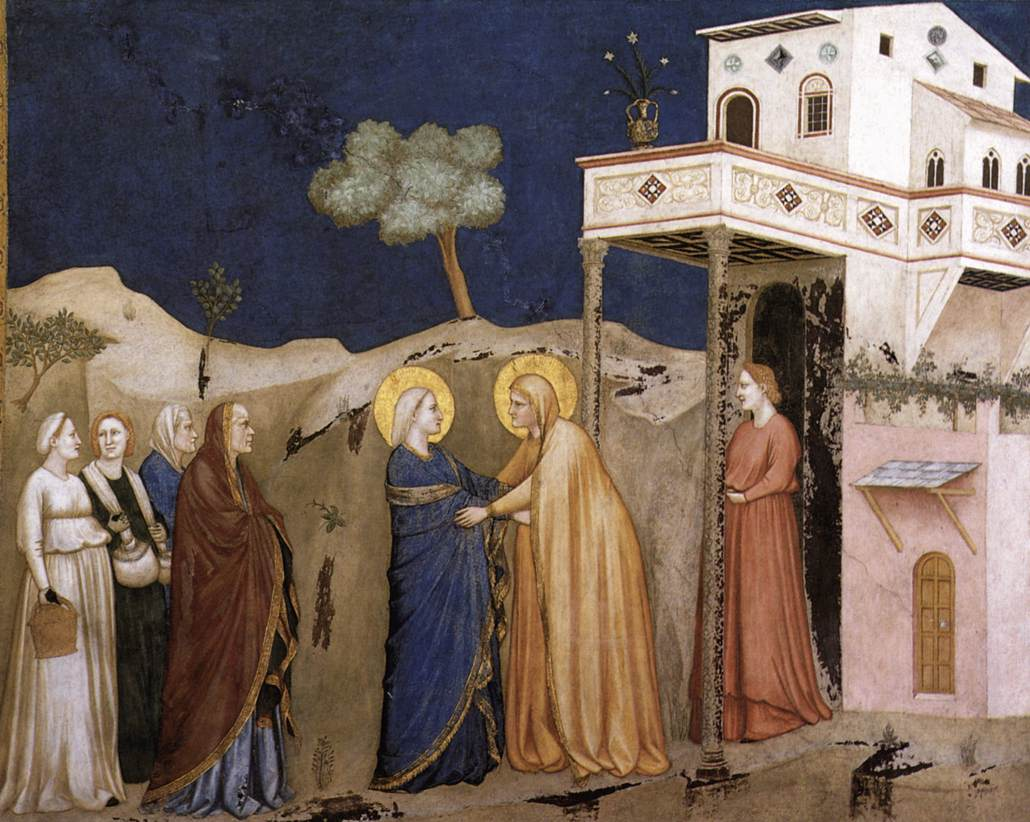
\includegraphics[width=\textwidth]{img/VisitationGiotto.jpg}

\addchap{Messe de la Visitation - 2 juillet}

\rubrica{ Le 2 juillet 1769, fête de la Visitation, un orage, tel qu'on n'en avait pas vu depuis longtemps, dévasta les campagnes de Saint-Cyprien, du Bugue, et de Terrasson. La paroisse de Tursac et le sanctuaire de Fontpeyrine furent seuls épargnés.
C'est pourquoi, les représentants de la ville de Tursac et sa pieuse population firent vœu d'aller au sanctuaire tous les ans en procession, au jour anniversaire du bienfait, pour remercier Notre-Dame de Fontpeyrine.}

\rubrica{La messe est à la page \emph{\pageref{Ordo}}, excepté les textes propres qui suivent~:}

\begin{multicols}{2}
\subsection*{Introït}
{Salut, ô Mère sainte~; mère qui avez enfanté le Roi qui régit le ciel et la terre dans les siècles des siècles.}
De mon cœur a jailli une parole excellente, c’est que je consacre mes œuvres à mon Roi. \vb\ Gloire au Père.

\subsection*{Collecte}
{Prions\\
Seigneur, nous vous prions d’accorder à vos serviteurs le don de la grâce céleste~: et, comme l’enfantement de la bienheureuse Vierge a été le principe de leur salut~; qu’ainsi la pieuse solennité de sa Visitation leur procure un accroissement de paix. Par Notre Seigneur.}
{\textbf{ \rb\ Amen.}}


\subsection*{Épître : Lecture du Livre de la Sagesse}
\rubrica{Cant. 2, 8-14.}
Voici qu’il vient, bondissant sur les montagnes, sautant sur les collines. Mon bien-aimé est semblable à la gazelle, ou au faon des biches. Le voici, il est derrière notre mur, regardant par la fenêtre, épiant par le treillis. Voici, mon bien-aimé me dit~: "Lève-toi, hâte-toi, mon amie, ma colombe, ma belle, et viens ! Car voici que l’hiver est fini~; la pluie a cessé, elle a disparu. Les fleurs ont paru sur notre terre, le temps des chants est arrivé~; la voix de la tourterelle s’est fait entendre dans nos campagnes~; le figuier pousse ses fruits naissants, les vignes en fleur donnent son parfum. Lève-toi, mon amie, ma belle, et viens ! Ma colombe, qui te tiens dans la fente du rocher, dans l’abri des parois escarpées, montre-moi ton visage, que ta voix résonne à mes oreilles~; car ta voix est douce, et ton visage charmant.
\textbf{\rb\ Deo grátias.}

\subsection*{Antiennes}
Vous êtes bénie et digne de vénération, Vierge Marie, qui avez été mère du Sauveur, sans que votre pureté ait subi d’atteinte. Vierge, Mère de Dieu, celui que tout l’univers ne peut contenir, s’est enfermé dans votre sein en se faisant homme.

Alléluia, alléluia. \vb\ Vous êtes heureuse, sainte Vierge Marie, et tout à fait digne de louange, car de vous est sorti le soleil de justice, le Christ notre Dieu. Alléluia.

\subsection*{Lecture du saint Évangile selon saint Luc.}
\rubrica{Luc 1, 39-47.}
En ces jours-là, Marie partit et s’en alla en hâte vers la montagne, en une ville de Juda. Et elle entra dans la maison de Zacharie, et salua Élisabeth. Or, quand Élisabeth entendit la salutation de Marie, l’enfant tressaillit dans son sein, et elle fut remplie du Saint-Esprit. Et elle s’écria à haute voix, disant~: "Vous êtes bénie entre les femmes, et le fruit de vos entrailles est béni. Et d’où m’est-il donné que la mère de mon Seigneur vienne à moi ? Car votre voix, lorsque vous m’avez saluée, n’a pas plus tôt frappé mes oreilles, que l’enfant a tressailli de joie dans mon sein. Heureuse celle qui a cru ! Car elles seront accomplies les choses qui lui ont été dites de la part du Seigneur !" Et Marie dit~: "Mon âme glorifie le Seigneur, et mon esprit tressaille de joie en Dieu, mon Sauveur".
{\textbf {\rb\ Laus tibi Christe.}}

\rubrica{Chant du Credo page \pageref{Credo}}

\subsection*{Antienne d'Offertoire}
Vous êtes bienheureuse, Vierge Marie, qui avez porté le Créateur de toutes choses ; vous avez enfanté celui qui vous a créée, et vous demeurez à jamais Vierge.

\subsection*{Oraison Secrète}
Qu’elle nous porte secours, Seigneur, la bonté de votre Fils unique, qui né d’une Vierge, n’a point altéré l’intégrité de sa Mère mais l’a consacrée, afin que nous purifiant de nos fautes en la solennité de sa Visitation, il vous rende notre oblation agréable, lui Jésus-Christ notre Seigneur.

\subsection*{Chant de communion}
Bienheureux le sein de la Vierge Marie, qui a porté le Fils du Père éternel.

\needspace{3\baselineskip}
\subsection*{Postcommunion}
{Nous avons reçu, Seigneur, les choses saintes qui vous sont offertes en cette solennité annuelle, faites, nous vous en supplions, qu’elles nous donnent les remèdes spirituels utiles à la vie temporelle et conduisant à la vie éternelle.}
\textbf{ \rb\ Amen.}

\end{multicols}

\addchap{Messe de l'Assomption - 15 août}

%\rubrica{ Le 2 juillet 1769, fête de la Visitation, un orage, tel qu'on n'en avait pas vu depuis longtemps, dévasta les campagnes de Saint-Cyprien, du Bugue, et de Terrasson. La paroisse de Tursac et le sanctuaire de Fontpeyrine furent seuls épargnés. C'est pourquoi, les représentants de la ville de Tursac et sa pieuse population firent vœu d'aller au sanctuaire tous les ans en procession, au jour anniversaire du bienfait, pour remercier Notre-Dame de Fontpeyrine.}

\rubrica{La messe est à la page \emph{\pageref{Ordo}} excepté les textes propres qui suivent~:}

\begin{multicols}{2}
\subsection*{Introït}
{Salut, ô Mère sainte~; mère qui avez enfanté le Roi qui régit le ciel et la terre dans les siècles des siècles.}
De mon cœur a jailli une parole excellente, c’est que je consacre mes œuvres à mon Roi. \vb\ Gloire au Père.

\subsection*{Collecte}
{Prions\\
Seigneur, nous vous prions d’accorder à vos serviteurs le don de la grâce céleste~: et, comme l’enfantement de la bienheureuse Vierge a été le principe de leur salut~; qu’ainsi la pieuse solennité de sa Visitation leur procure un accroissement de paix. Par Notre Seigneur.}
{\textbf \rb\ Amen.}

\subsection*{Antiennes}
Vous êtes bénie et digne de vénération, Vierge Marie, qui avez été mère du Sauveur, sans que votre pureté ait subi d’atteinte. Vierge, Mère de Dieu, Celui que tout l’univers ne peut contenir, s’est enfermé dans votre sein en se faisant homme.

Alléluia, alléluia. \vb\ Vous êtes heureuse, sainte Vierge Marie, et tout à fait digne de louange, car de vous est sorti le soleil de justice, le Christ notre Dieu. Alléluia.

\subsection*{Epître : Lecture du Livre de la Sagesse.}
\rubrica{Cant. 2, 8-14.}
Voici qu’il vient, bondissant sur les montagnes, sautant sur les collines. Mon bien-aimé est semblable à la gazelle, ou au faon des biches. Le voici, il est derrière notre mur, regardant par la fenêtre, épiant par le treillis. Voici, mon bien-aimé me dit~: "Lève-toi, hâte-toi, mon amie, ma colombe, ma belle, et viens ! Car voici que l’hiver est fini~; la pluie a cessé, elle a disparu. Les fleurs ont paru sur notre terre, le temps des chants est arrivé~; la voix de la tourterelle s’est fait entendre dans nos campagnes~; le figuier pousse ses fruits naissants, les vignes en fleur donnent son parfum. Lève-toi, mon amie, ma belle, et viens ! Ma colombe, qui te tiens dans la fente du rocher, dans l’abri des parois escarpées, montre-moi ton visage, que ta voix résonne à mes oreilles~; car ta voix est douce, et ton visage charmant.
\textbf{\rb\ Deo grátias.}

\subsection*{Lecture du Saint Évangile selon saint Luc.}
\rubrica{Luc. 1, 39-47.}
En ces jours-là~: Marie partit et s’en alla en hâte vers la montagne, en une ville de Juda. Et elle entra dans la maison de Zacharie, et salua Élisabeth. Or, quand Élisabeth entendit la salutation de Marie, l’enfant tressaillit dans son sein, et elle fut remplie du Saint-Esprit. Et elle s’écria à haute voix, disant~: "Vous êtes bénie entre les femmes, et le fruit de vos entrailles est béni. Et d’où m’est-il donné que la mère de mon Seigneur vienne à moi ? Car votre voix, lorsque vous m’avez saluée, n’a pas plus tôt frappé mes oreilles, que l’enfant a tressailli de joie dans mon sein. Heureuse celle qui a cru ! Car elles seront accomplies les choses qui lui ont été dites de la part du Seigneur !" Et Marie dit~: "Mon âme glorifie le Seigneur, et mon esprit tressaille de joie en Dieu, mon Sauveur".
{\textbf \rb\ Laus tibi Christe.}

\subsection*{Antienne d'offertoire}
Vous êtes bienheureuse, Vierge Marie, qui avez porté le Créateur de toutes choses ; vous avez enfanté celui qui vous a créée, et vous demeurez à jamais Vierge.

\subsection*{Oraison Secrète}
Qu’elle nous porte secours, Seigneur, la bonté de votre Fils unique, qui né d’une Vierge, n’a point altéré l’intégrité de sa Mère mais l’a consacrée, afin que nous purifiant de nos fautes en la solennité de sa Visitation, il vous rende notre oblation agréable, lui Jésus-Christ Notre-Seigneur.

\subsection*{Chant de communion}
Bienheureux le sein de la Vierge Marie, qui a porté le Fils du Père éternel.

\subsection*{Postcommunion}
{Nous avons reçu, Seigneur, les choses saintes qui vous sont offertes en cette solennité annuelle, faites, nous vous en supplions, qu’elles nous donnent les remèdes spirituels utiles à la vie temporelle et conduisant à la vie éternelle.}
{\textbf \rb\ Amen.}

\addchap{Messe de la Nativité de la Vierge - 8 septembre}

\rubrica{Avant la proclamation du dogme de l'Immaculé Conception (1854) et sa fête le 8 décembre, la fête de la Nativité de la Vierge était celle qui commémorait cette vérité si importante : que le péché n'a pas atteint Marie, même pas le péché originel. Elle naît donc immaculée, et voilà pourquoi nous fêtons sa naissance.}

\rubrica{À Fontpeyrine, comme de nombreux sanctuaires périgourdins et français (Capelou, Laveyssière, Sanilhac, Redon-Espic, …), c'est aujourdhui la fête patronale.}

\rubrica{La messe est à la page \emph{\pageref{Ordo}}, excepté les textes propres qui suivent~:}

\begin{multicols}{2}
\subsection*{Introït}
Salut, ô Mère sainte ; mère qui avez enfanté le Roi qui régit le ciel et la terre dans les siècles des siècles.
De mon cœur a jailli une parole excellente, c’est que je consacre mes œuvres à mon Roi.
\vb\ Gloire au Père.

\subsection*{Collecte}
Prions\\
Seigneur, nous vous prions d’accorder à vos serviteurs le don de la grâce céleste ; et, comme l’enfantement de la bienheureuse Vierge a été le principe de leur salut, qu’ainsi la pieuse solennité de sa Nativité leur procure un accroissement de paix.
{\textbf {\rb\ Amen.}}

\subsection*{Épître : Lecture du Livre des Proverbes}
\rubrica{Prov. 8, 22-35.}
Le Seigneur m’a possédée au commencement de ses voies, avant de faire quoi que ce soit, dès le principe. J’ai été établie dès l’éternité, et dès les temps anciens, avant que la terre fût créée. Les abîmes n’étaient pas encore, et déjà j’étais conçue ; les sources des eaux n’avaient pas encore jailli ; les montagnes ne s’étaient pas encore dressées avec leur pesante masse ; j’étais enfantée avant les collines. Il n’avait pas encore fait la terre, ni les fleuves, ni les bases du globe terrestre. Lorsqu’il préparait les cieux, j’étais là ; lorsqu’il environnait les abîmes de leurs bornes, par une loi inviolable ; lorsqu’il affermissait l’air dans les régions supérieures, et qu’il équilibrait les sources des eaux ; lorsqu’il entourait la mer de ses limites, et qu’il imposait une loi aux eaux, pour qu’elles ne franchissent point leurs bornes, lorsqu’il posait les fondements de la terre, j’étais avec lui, réglant toutes choses, et j’étais chaque jour dans les délices, me jouant sans cesse devant lui, me jouant sur le globe de la terre, et mes délices sont d’être avec les enfants des hommes. Maintenant donc, mes fils, écoutez-moi : Heureux ceux qui gardent mes voies. Écoutez mes instructions et soyez sages, et ne les rejetez pas. Heureux l’homme qui m’écoute, et qui veille tous les jours à ma porte, et qui se tient à la porte de ma maison. Celui qui me trouvera, trouvera la vie, et puisera le salut dans le Seigneur.
\textbf{\rb\ Deo grátias.}

\subsection*{Antiennes}
Vous êtes bénie et digne de vénération, Vierge Marie, qui avez été mère du Sauveur, sans que votre pureté ait subi d’atteinte.
\vb Vierge, Mère de Dieu, celui que tout l’univers ne peut contenir, s’est enfermé dans votre sein en se faisant homme.

Allelúia, allelúia. \vb\ Vous êtes heureuse, sainte Vierge Marie, et tout à fait digne de louange, car de vous est sorti le soleil de justice, le Christ notre Dieu. Alléluia.

\subsection*{Début du Saint Évangile selon saint Mathieu}
\rubrica{Matth. 1, 1-16.}
Généalogie de Jésus-Christ, fils de David, fils d’Abraham. Abraham engendra Isaac ; Isaac engendra Jacob ; Jacob engendra Juda et ses frères ; Juda, de Thamar, engendra Pharès et Zara ; Phares engendra Esrom ; Esrom engendra Aram ; Aram engendra Aminadab ; Aminadab engendra Naasson ; Naasson engendra Salmon ; Salmon, de Rahab, engendra Booz ; Booz, de Ruth, engendra Obed ; Obed engendra Jessé ; Jessé engendra le roi David. David engendra Salomon de la femme d’Urie ; Salomon engendra Roboam ; Roboam engendra Abia ; Abia engendra Asa ; Asa engendra Josaphat ; Josaphat engendra Joram ; Joram engendra Ozias ; Ozias engendra Joatham ; Joatham engendra Achaz ; Achaz engendra Ezéchias ; Ezéchias engendra Manassé ; Manassé engendra Amon ; Amon engendra Josias ; Josias engendra Jéchonias et ses frères, au temps de la déportation à Babylone. Après la déportation à Babylone, Jéchonias engendra Salathiel ; Salathiel engendra Zorobabel ; Zorobabel engendra Abioud ; Abioud engendra Eliacim ; Eliacim engendra Azor ; Azor engendra Sadoc ; Sadoc engendra Achim ; Achim engendra Elioud ; Elioud engendra Eléazar ; Eléazar engendra Matthan ; Matthan engendra Jacob ; Jacob engendra Joseph l’époux de Marie, de laquelle est né Jésus, qu’on appelle Christ.
\textbf{ \rb\ Laus tibi Christe.}


\rubrica{Chant du Credo page \pageref{Credo}}

\subsection*{Antienne d'Offertoire}
Vous êtes bienheureuse, Vierge Marie, qui avez porté le Créateur de toutes choses ; vous avez enfanté celui qui vous a créée, et vous demeurez à jamais Vierge.

\subsection*{Oraison Secrète}
Qu’elle nous porte secours, Seigneur, la bonté de votre Fils unique, qui né d’une Vierge, n’a point altéré l’intégrité de sa mère mais l’a consacrée, afin que nous purifiant de nos fautes en la solennité de sa Nativité, il vous rende notre oblation agréable, lui Jésus-Christ notre Seigneur.

\subsection*{Chant de Communion}
Bienheureux le sein de la Vierge Marie, qui a porté le Fils du Père éternel.

\subsection*{Postcommunion}
Nous avons reçu, Seigneur, les choses saintes qui vous sont offertes en cette solennité annuelle, faites, nous vous en supplions, qu’elles nous donnent les remèdes spirituels utiles à la vie temporelle et conduisant à la vie éternelle.
\textbf{ \rb\ Amen.}
\end{multicols}

\clearpage
\addchap{Kyriale}
\section{Kyriale VIII}
\cantus{Kyriale}{Kyrie-VIII}{}{5.}
\cantus{Kyriale}{Gloria-VIII}{}{5.}
\cantus{Kyriale}{Sanctus-VIII}{}{6.}
\cantus{Kyriale}{Agnus-VIII}{}{6.}
\cantus{Kyriale}{Ite-VIII}{}{5.}
\culdelampe{3cm}{img/CulsDeLampe/foliage.pdf}

\section{Kyriale IX}
\cantus{Kyriale}{Kyrie-IX}{}{1.}
\cantus{Kyriale}{Gloria-IX}{}{7.}
\cantus{Kyriale}{Sanctus-IX}{}{5.}
\cantus{Kyriale}{Agnus-IX}{}{1.}
\cantus{Kyriale}{Ite-IX}{}{1.}
\begin{center}

\includegraphics[width=3cm]{img/CulsDeLampe/foliage.pdf}
\end{center}

\section[Credo]{Credo III}
\label{Credo}
\cantus{Kyriale}{Credo-III}{}{5.}

\culdelampe{5cm}{img/CulsDeLampe/rosace-4.pdf}

\newcommand{\commandement}[1]{\noindent\textbf{#1}}
\addchap{Sacrement de Pénitence}

Le sacrement de Pénitence ou confession fut institué par Notre Seigneur Jésus-Christ, pour effacer les péchés commis après le baptême. Notre-Seigneur l’a transmis aux Apôtres lorsqu’il leur a dit : « Recevez le Saint-Esprit ; les péchés seront remis à ceux à qui vous les remettrez et ils seront retenus à ceux à qui vous les retiendrez. »


\addsec[Pour les enfants]{\underline{Pour les enfants}}

Pour bien recevoir le sacrement de Pénitence, il faut connaître ses péchés, en avoir la contrition, les accuser, et après en avoir reçu l’absolution, faire la pénitence imposée par le prêtre.

\subsection*{Qu’est-ce que se confesser ?}

C’est dire ses péchés à un prêtre pour en recevoir l’absolution.

\subsection*{Comment se confesser ?}

Deux choses à faire :
\begin{itemize}
\item retrouver nos péchés ;
\item les regretter.
\end{itemize}

\emph{Pour les chercher}, fermons les yeux et faisons l’examen de conscience. Nous pouvons nous aider de l’examen de conscience qui suit.
\pagebreak[3]

\emph{Pour les regretter}, disons lentement :\\
Esprit-Saint, qui êtes la lumière de nos cœurs, éclairez ma conscience, montrez-moi mes péchés, faites que je les voie, comme je les verrai à l’heure de mon jugement et comme les voyait Jésus, quand il mourait pour les réparer. Montrez-moi les défauts qui m’ont poussé à les commettre, pour que je les combatte. Faites que je sois bien décidé à suivre les conseils de votre prêtre, pour que votre grâce en moi rencontre moins d’obstacles, et puisse me guérir de mes mauvais penchants. Ainsi-soit-il !

\subsection*{Examen de conscience}

\minisec{Confession précédente}

\begin{itemize}
\item Combien y a-t-il de temps que je ne me suis pas confessé ?
\item Ai-je bien dit tous mes péchés ?
  \begin{itemize}
  \item N’ai-je pas caché volontairement des péchés graves ? (Si oui, il vous faut absolument vous en accuser, car non seulement aucun de vos péchés accusés n’a été pardonné, mais vous avez ajouté un autre péché très grave : un sacrilège).
  \item N’ai-je pas oublié des péchés graves ? (Si oui, votre dernière confession a été bonne quand même ; mais il faut que vous les accusiez maintenant).
  \end{itemize}
\item Me suis-je mal préparé à ma dernière confession ?
\item N’ai-je pas manqué de contrition, c’est-à-dire de vrai repentir de mes fautes ? (pour avoir un vrai repentir, il faut être décidé à faire tout son possible pour ne pas recommencer).
\item Ai-je fait ma pénitence ?
\item Quelle résolution avais-je prise lors de ma dernière confession ? Est-ce que je l’ai tenue ?
\end{itemize}

\needspace{3\baselineskip}
\minisec{Commandements de Dieu}

\commandement{1. Tu adoreras Dieu seul et tu l'aimeras plus que tout.}

\begin{itemize}
\item Ai-je manqué mes prières ? du matin ? du soir ? les ai-je mal faites ?
\item Me suis-je mal tenu à l’église ? Ai-je dissipé les autres ?
\item Ai-je eu honte de paraître chrétien ?
\item Ai-je tenu des conversations contre la religion ?
\end{itemize}

\commandement{2. Tu ne prononceras le nom de Dieu qu’avec respect.}
\begin{itemize}
\item Ai-je dit des gros mots ? Ai-je dit des jurons ?
\item Ai-je fait des serments pour des riens ?
\end{itemize}

\commandement{3. Tu sanctifieras le jour du Seigneur.}
\begin{itemize}
\item Ai-je manqué par ma faute, la messe le dimanche ou les fêtes d’obligation ? Combien de fois ?
\item Suis-je arrivé en retard ? À quel moment ?
\end{itemize}

\commandement{4. Tu honoreras ton père et ta mère.}
\begin{itemize}
\item Ai-je désobéi à mes parents ?
\item Leur ai-je mal répondu ? Me suis-je moqué d’eux ?
\item Ai-je fait la tête ? Ai-je fait du mauvais esprit ?
\end{itemize}

\commandement{5. Tu ne tueras pas.}
\begin{itemize}
\item Me suis-je disputé avec les autres ?
\item Ai-je gardé rancune ? Ai-je cherché à me venger ?
\item Ai-je donné le mauvais exemple ? ou entraîné d’autres à pécher ?
\end{itemize}

\commandement{6. Tu ne feras pas d'impureté.\\
9. Tu n'auras pas de désir impur volontaire.}
\begin{itemize}
\item Ai-je regardé des images mauvaises, impures ? Ai-je cherché exprès des journaux impurs ?
\item Ai-je vu des spectacles mauvais (à la télévision par exemple) ?
\item Ai-je accepté des pensées impures ? des désirs impurs ?
\item Ai-je participé à de mauvaises conversations ?
\item Ai-je fait des actions impures ? seul ? avec d’autres ?
\end{itemize}

\commandement{7. Tu ne voleras pas.\\
10. Tu ne désireras pas injustement le bien des autres.}
\begin{itemize}
\item Ai-je pris ou recherché à prendre quelque chose qui n’était pas à moi (des gourmandises, de l’argent) ?
\item Ai-je abîmé exprès ce qui ne m’appartenait pas ?
\item Ai-je triché au jeu ? Ai-je copié en classe, à un examen, à une composition, à un devoir ?
\end{itemize}

\commandement{8. Tu ne mentiras pas.}
\begin{itemize}
\item Ai-je menti ? (pour m’amuser, pour me vanter, pour ne pas être puni, pour tromper).
\item Ai-je dit du mal des autres ? Ai-je cherché à faire punir les autres ?
\item  Ai-je pensé sans raison suffisante, du mal des autres ?
\end{itemize}


\needspace{3\baselineskip}
\minisec{Commandements de l'Église}

\begin{itemize}
\item Me suis-je bien préparé à ma dernière
 communion ?
\item Ai-je communié sans être à jeun ?
\item Ai-je communié avec des péchés graves sur la conscience ?
\item Ai-je mangé de la viande les jours défendus ?
\end{itemize}


\needspace{3\baselineskip}
\minisec{Péchés capitaux}

\begin{itemize}
\item Ai-je été orgueilleux ? Ai-je refusé de reconnaître mes torts ? Ai-je rabaissé les autres en pensée ? Me suis-je vanté ? Me suis-je vexé pour rien ?
\item Ai-je été gourmand : en étant difficile ? en mangeant trop de friandises ? en
mangeant et en buvant avec excès ? Ai-je fumé en cachette ?
\item Ai-je été avare ? Ai-je refusé de prêter mes affaires ?
\item Ai-je été jaloux ?
\item Me suis-je mis en colère ? Ai-je eu mauvais caractère, rendant la vie pénible
autour de moi ? Ai-je été impatient ? Ai-je fait mettre exprès les autres en colère ?
\item Ai-je été paresseux ? pour me lever ? pour prier ? pour communier ? à l’école ? au catéchisme ? pour faire mes devoirs ? Ai-je manqué par ma faute l’école ou le catéchisme ?
\end{itemize}

Mon défaut dominant est : …

Je prends la résolution de : …


\addsec[Pour les adultes]{\underline{Pour les adultes}}

Le sacrement de Pénitence, appelé aussi confession, est le sacrement institué par Jésus-Christ pour remettre les péchés commis après le baptême. Le ministre de ce sacrement est le prêtre. Tenant la place de Jésus-Christ et recevant la confidence de nos péchés même les plus cachés, le prêtre est tenu à un secret absolu sur tout ce qu’il a entendu. C’est le secret de confession. Même sous la menace de mort ou de torture, il ne peut rien dire et rien révéler. Nous pouvons donc lui parler en toute confiance et sans crainte.

Ce sacrement exige quatre conditions :
\begin{enumerate}
\item la connaissance de nos péchés ;
\item la contrition de nos péchés ;
\item la confession de nos péchés au prêtre suivie de l’absolution ;
\item la satisfaction pour nos péchés.
\end{enumerate}

\smallskip
Les parties du sacrement sont :
\begin{itemize}
\item la contrition : c’est un acte de volonté, une douleur de l’âme et l’horreur du péché commis, et la résolution de ne plus pécher à l’avenir ;
\item la confession : elle consiste dans l’accusation détaillée de nos péchés faite au confesseur pour en avoir l’absolution et la pénitence ;
\item l'absolution : c’est la phrase que le prêtre prononce au nom de Jésus-Christ, pour remettre les péchés au pénitent ;
\item la satisfaction : ou pénitence sacramentelle, c’est la prière ou la bonne œuvre imposée par le confesseur pour le châtiment et la correction du pêcheur, et l’escompte de la peine temporelle méritée en péchant.
\end{itemize}

\smallskip
\textbf{Les effets de la confession bien faite} : le sacrement de Pénitence :
\begin{itemize}
\item donne la grâce sanctifiante avec laquelle les péchés mortels, et aussi les péchés véniels, confessés et que l'on regrette, nous sont remis ;
\item commue la peine éternelle en temporelle ; celle-ci est diminuée dans la mesure de la contrition ;
\item rend les mérites des bonnes œuvres faites avant de commettre le péché
mortel ;
\item donne à l’âme les secours nécessaires pour ne pas retomber dans le péché et redonner la paix à la conscience.
\end{itemize}

\smallskip
\textbf{Pour préparer une bonne confession :}

dans la confession il faut accuser au moins tous les péchés mortels, pas encore bien confessés (dans une bonne confession) et ceux que l’on se rappelle. Indiquer, dans la mesure du possible, leur espèce et leur nombre.

Pour cela on demande à Dieu la grâce de bien connaître ses fautes, et on s’examine sur les dix commandements et les préceptes de l’Église, sur les péchés capitaux et les devoirs de notre état.

N.B. 1. Pour reconnaître un péché mortel (c’est-à-dire qui donne la mort surnaturelle à l’âme), il faut trois choses :
\begin{itemize}
\item la gravité de la matière ;
\item la pleine advertance (c’est-à-dire la pleine connaissance) ;
\item le plein consentement.
\end{itemize}

2. L’accusation de l’espèce et du nombre est de rigueur pour les désirs, au moins approximativement s'il n'est pas possible de se souvenir du nombre exact.


\subsection*{Examen de conscience}

\minisec{Commandements de Dieu}

\commandement{1. Tu adoreras Dieu seul et tu l'aimeras plus que tout.}

Manqué à mes prières, les ai mal faites.
Craint de me montrer chrétien, par respect humain. Négligé de m’instruire des
vérités de la religion, doutes volontaires.
Lu des livres, des journaux impies. Parlé,
agi contre la religion. Murmuré contre
Dieu et sa Providence. Appartenu à des
sociétés impies (franc-maçonnerie, communisme, sectes hérétiques, etc.) Pratiqué
des superstitions, consulté les cartes et les
devins. Avoir tenté Dieu.

Péchés contre la foi : refuser d’admettre
une ou plusieurs vérités révélées de Dieu.
Péchés contre l’espérance : manquer de
confiance en la bonté et Providence de
Dieu. Prétendre qu’il soit impossible de
vivre en vrai chrétien quoiqu’on en demande la grâce. Pécher par présomption
en abusant de la bonté de Dieu.

Péchés contre la charité : refuser d’aimer
Dieu par-dessus tout. Passer des semaines
et des mois sans faire le plus petit acte
d’amour de Dieu. Indifférence religieuse.
Sacrilèges en profanant les choses saintes,
en particulier confessions et communions
sacrilèges.

Charité envers le prochain : refuser de
voir Dieu dans nos frères, d’aimer Dieu
dans le prochain. Mépriser, détester, se
moquer du prochain.

\commandement{2. Tu ne prononceras le nom de Dieu qu’avec respect.}

Fait des serments faux ou inutiles — Imprécations contre moi-même ou contre
d’autres — Manqué de respect à l’égard
du nom de Dieu ou des saints — Blasphémé en murmurant contre Dieu dans
les épreuves — Manqué à des vœux.

\commandement{3. Tu sanctifieras le jour du Seigneur.}

À ce commandement se rapportent les 1\ier\ et 2\ieme\ commandements de l’Église.
Manqué à la messe le dimanche par ma faute, arrivé
en retard, assisté sans respect. Travaillé
ou fait travailler sans nécessité et sans
permission. Avoir profané
cette journée par des réunions ou amusements dangereux pour la foi ou les
mœurs.

\commandement{4. Tu honoreras ton père et ta mère.}

Enfants : manqué de respect. Désobéi.
Causé du chagrin à mes parents. Négligé
de les assister. N’avoir pas tenu compte de
leurs sages avis.

Parents : ai-je pensé à donner ou procurer
une instruction religieuse à nos enfants ?
Les ai-je fait prier ? Ai-je choisi pour eux
l’école la plus sûre ? Veillé sur eux avec
diligence ? Les ai-je conseillés, repris,
corrigés ?

Époux : l’amour entre les conjoints est-il
vraiment patient, empressé, prêt à tout ?
Manque de support mutuel. Avoir critiqué
son conjoint devant les enfants.

Inférieurs (employés, ouvriers, soldats) :
manque de respect, d’obéissance à mes
supérieurs — Fait du tort par des critiques
— Négligé mon service. Commis des abus
de confiance.

Supérieurs : manqué à la justice commutative, en ne donnant pas ce qui était dû, à
la justice sociale. Manqué à la charité, en
ne procurant pas les secours nécessaires
— N’avoir pas traité ses employés avec
bonté, équité, charité.

\commandement{5. Tu ne tueras pas.}

M’être mis en colère. Voulu me venger.
Souhaité du mal — Haines, rancunes, refuser de pardonner — Ai injurié, blessé
— Impatiences ­ — Mauvais conseils —
Scandalisé par paroles... actions — Infanticide — Avortement — Euthanasie —
Transgressions graves au code de la route,
de façon volontaire (même s’il n’est rien
arrivé).

\commandement{6. Tu ne feras pas d'impureté.\\
9. Tu n'auras pas de désir impur volontaire.}

M’être arrêté volontairement à des pensées, à des désirs contraires à la pureté
— Conversations et chansons légères ou
déshonnêtes, vêtements indécents — Télévision, radio (mauvaises émissions),
gravures, livres, journaux mauvais — Regards, familiarités coupables — Actions
déshonnêtes, seul... avec d’autres —
Liaisons ou fréquentations coupables —
Fraudes dans l’usage du mariage — Refus
du dû conjugal — Péchés entre fiancés.

\commandement{7. Tu ne voleras pas.\\
10. Tu ne désireras pas injustement le bien des autres.}

Désiré prendre le bien d’autrui ­ — Commis ou aidé à commettre des injustices,
des fraudes, des vols — Causé du dommage — Pas restitué — Pas payé mes dettes — Fait tort dans les ventes, contrats,
transactions, etc.

\commandement{8. Tu ne mentiras pas.}

Ai menti — Jugé témérairement — Dit
du mal du prochain — Calomnié — Faux
témoignage — Violé des secrets (lu une
lettre). Fait ou diffusé des soupçons.


\minisec{Commandements de l'Église}

\commandement{1. Les fêtes tu sanctifieras qui te sont de commandement.\\
2. Les dimanches Messe tu entendras, et les fêtes pareillement.}

Voir au 3\ieme\ commandement de Dieu.

\commandement{3. Tous tes péchés confesseras, à tout le moins une fois l’an.\\
4. Ton Créateur tu recevras, au moins à Pâques humblement.}

Être resté plus d'un an sans confesser un péché grave. Ne pas avoir communié, au moins à Pâques. Avoir fait des communions sacrilèges.

\commandement{5. Vigiles, pénitence feras − Carême et Quatre-Temps également.\\
6. De la viande ne mangeras les jours défendus mêmement.}

Avoir sans raison légitime et sans permission : manqué au jeûne - mangé de la viande les jours défendus - manqué au
jeûne eucharistique.

\commandement{7. Loi de l'Index}

Avoir lu ou conservé des livres, revues ou journaux défendus expressément par l’Église ou contre la foi et les mœurs.


\minisec{Péchés capitaux}

\commandement{Orgueil}

Agi par orgueil - Dépenses et luxes exagérés - Méprisé les autres - M’être complu
dans des pensées de vanité - Susceptibilités - Être esclave du « qu’en dira-t-on ? »
et la mode.

\commandement{Avarice}

M’être trop attaché à l’argent - N’avoir
pas fait l’aumône selon mes moyens - Jeux
d’argent (voir aux 7\ieme\ et 10\ieme\ commandements
de Dieu).

\commandement{Luxure} : voir aux 6\ieme\ et 9\ieme\ commandements de Dieu.

\commandement{Envie}

Avoir entretenu des sentiments de jalousie - Cherché à nuire aux autres par envie
- M’être réjoui du mal ou attristé du bien
d’autrui.

\commandement{Gourmandise}

Excès dans le manger, dans le boire.
Ivresse : combien de fois ? Usage de stupéfiants.

\commandement{Colère} : voir au 5\ieme\ commandement de Dieu.

\commandement{Paresse}

Au lever. Dans le travail. Dans les devoirs religieux.

\clearpage
\tableofcontents
\printindex

\newpage
\thispagestyle{empty}
\vspace*{\stretch{1}}
{\centering{Si vous voulez nous aider, vous pouvez adresser vos dons à :

\smallskip
\textsc{Association Notre-Dame de Fontpeyrine}


\textit{adresse administrative :}\\
5, rue de Clairat\\
24100 BERGERAC\\
\smallskip

Ordre des chèques : « Notre-Dame de Fontpeyrine »\\
}
}
\vspace*{\stretch{1}}
\newpage

%\vfill\thispagestyle{empty}

{\thispagestyle{empty}\centering
\vspace*{\stretch{2}}


\includegraphics[width=.6\textwidth]{img/SceauJubile.pdf}

{\centering {\textit{Notre-Dame de Fontpeyrine,\\
qui depuis des
siècles 
accordez de nombreuses faveurs\\
à ceux qui ont recours à votre puissante intercession,\\
obtenez, nous vous en supplions,\\
à nous vos humbles serviteurs, \\
en souvenir de votre bienheureuse Nativité,\\
ce complément de grâce\\
que nous implorons à genoux devant vous.\\
Nous l’attendons avec confiance,\\
malgré notre indignité, ô Mère du Sauveur,\\
de votre maternelle bonté\\
et de votre bienveillante protection.\\
Ainsi soit-il.\\}}}

\vspace*{\stretch{3}}

\footnotesize Association N-D. de Fontpeyrine\\
Aumônerie assurée par la Fraternité Sacerdotale Saint-Pie X\par}
\end{document}